\documentclass[format=sigconf,10pt,natbib=false]{acmart}
\usepackage{geometry}
%\topmargin -0.5in
%\headheight 0pt
%\textheight 9.25in
%\settopmatter{printacmref=false}

% remove the annoying header on each page
%\fancyhead{}

\if 0
\setlength\paperheight{11in}
\setlength\paperwidth{8.5in}
\setlength{\textwidth}{7in}
\setlength{\textheight}{9.25in}
\setlength{\oddsidemargin}{-.25in}
\setlength{\evensidemargin}{-.25in}

\fi

%
\usepackage{xspace}
\usepackage{multirow}
\usepackage{comment}
\usepackage{fancybox, fancyvrb, calc}
\usepackage{subcaption}
\usepackage[inline]{enumitem}
\usepackage{amsmath, amssymb}
\usepackage{cite,url}
\usepackage{pbox}
\usepackage{balance}
\usepackage{wrapfig}
%
%\usepackage[T1]{fontenc}
\usepackage[utf8]{inputenc}
\usepackage{mathptmx}
\usepackage{enumitem}
\setlist{nolistsep}
\usepackage{hhline}
%
\captionsetup[table]{skip=-1pt,font={footnotesize}}
\captionsetup[subfigure]{skip=-1pt,font={footnotesize}}
\captionsetup[figure]{font={footnotesize}}
\Urlmuskip=0mu plus 1mu
\hypersetup{%
  colorlinks=true,      % false: boxed links; true: colored links
  linkcolor=blue,       % color of internal links
  citecolor=magenta,    % color of links to bibliography
  filecolor=cyan,       % color of file links
  urlcolor=blue          % color of external links
}
%
\usepackage{leading}
\leading{12pt}
%
\usepackage{minted}
\usepackage{listings}
\lstset{
  columns=flexible,
  mathescape,
  keepspaces=true,
  escapeinside={(*}{*)},
  basicstyle=\ttfamily\small  
}
%
%\usepackage[subtle]{savetrees}
\usepackage[small,compact]{titlesec}
\usepackage{outlines}
%
\newcommand{\cut}[1]{}
%
\newcommand{\paragraphnone}[1]{\vspace{0.075in}\noindent{\bf #1}}
\newcommand{\paragrapha}[1]{\vspace{0.075in}\noindent{\bf #1.}}
\newcommand{\paragraphq}[1]{\vspace{0.075in}\noindent{\bf #1}}
%
\newcommand{\eg}{e.g., }
\newcommand{\etc}{{etc.}\xspace}
\newcommand{\ie}{i.e., }
\newcommand{\ccp}{CCP\xspace}
%
\newcommand{\an}[1]{{\color{green}\bf AN: {#1}}}
\newcommand{\sn}[1]{{\color{purple}\bf NG: {#1}}}
\newcommand{\hb}[1]{{\color{brown}\bf HB: {#1}}}
\newcommand{\ma}[1]{{\color{red}\bf MA: {#1}}}
\newcommand{\pg}[1]{{\color{blue}\bf PG: {#1}}}
\newcommand{\fc}[1]{{\color{blue}\bf FC: {#1}}}
\newcommand{\dr}[1]{{\color{magenta}\bf DR: {#1}}}
\newcommand{\radhika}[1]{{\color{cyan}\bf RM: {#1}}}
%
\newcommand{\datapath}{datapath\xspace}
\newcommand{\datapaths}{datapaths\xspace}
\newcommand{\Datapaths}{Datapaths\xspace}
\newcommand{\Datapath}{Datapath\xspace}
%
\frenchspacing
%
\newcommand{\handlers}{callbacks\xspace}
\newcommand{\userspace}{user-space\xspace}
\newcommand{\kernelspace}{kernel-space\xspace}
%
\newcommand{\controller}{agent\xspace}

\newcommand{\ct}[1]{{\tt #1}}
\newcommand{\ngs}[1]{{\textcolor{red}{NG: #1}}}
\newcommand{\Para}[1]{\vspace{4pt}\noindent{\bf #1}}
\newcommand{\Sec}[1]{\S\ref{#1}}

%\captionsetup[figure]{belowskip=-5pt, aboveskip=5pt}
%\setlength{\abovedisplayskip}{0pt}
%\setlength{\belowdisplayskip}{-5pt}

\begin{document}
\title{Restructuring Endpoint Congestion Control}
\author{Akshay Narayan, Frank Cangialosi, Deepti Raghavan, Prateesh Goyal}
\author{Srinivas Narayana, Radhika Mittal, Mohammad Alizadeh, Hari Balakrishnan}
\email{ccp@csail.mit.edu}
\affiliation{MIT Computer Science and Artificial Intelligence Laboratory}
%\email{{akshayn,frankc,deeptir,prateesh,alephtwo,alizadeh,hari}@csail.mit.edu, radhika@eecs.berkeley.edu}
\begin{CCSXML}
<ccs2012>
<concept>
<concept_id>10003033.10003039.10003048</concept_id>
<concept_desc>Networks~Transport protocols</concept_desc>
<concept_significance>500</concept_significance>
</concept>
<concept>
<concept_id>10003033.10003039.10003040</concept_id>
<concept_desc>Networks~Network protocol design</concept_desc>
<concept_significance>300</concept_significance>
</concept>
</ccs2012>
\end{CCSXML}
\acmYear{2018}\copyrightyear{2018}
\setcopyright{acmlicensed}
\acmConference[SIGCOMM '18]{SIGCOMM '18: SIGCOMM 2018}{August 20--25, 2018}{Budapest, Hungary}
\acmBooktitle{SIGCOMM '18: SIGCOMM 2018, August 20--25, 2018, Budapest, Hungary}
\acmPrice{15.00}
\acmDOI{10.1145/3230543.3230553}
\acmISBN{978-1-4503-5567-4/18/08}
\ccsdesc[500]{Networks~Transport protocols}
\ccsdesc[300]{Networks~Network protocol design}
\keywords{Congestion control, Operating systems}

% fix right arrow in CCS keywords
\settopmatter{printacmref=false} % Removes citation information below abstract
\newcommand*{\origrightarrow}{$\rightarrow$}
\let\oldarrow\textrightarrow
\renewcommand*{\textrightarrow}{\fontfamily{cmr}\selectfont\origrightarrow}
%\renewcommand{\shortauthors}{Akshay Narayan, Frank Cangialosi, Deepti Raghavan, et al.}
\renewcommand{\shortauthors}{}

\begin{sloppypar}
\begin{abstract}

This paper describes the implementation and evaluation of a Congestion Control Plane (CCP), a new way to structure congestion control functions at the sender by removing them from the datapath. With CCP, each datapath such as the Linux Kernel TCP, UDP-based QUIC, or kernel-bypass transports like mTCP/DPDK summarizes information about the round-trip time, packet receptions, losses, ECN, etc. via a well-defined interface, and algorithms running atop CCP can use this information to control the datapath's congestion window or pacing rate. We show that CCP enables, for the first time, congestion control algorithms to be written once and run on multiple datapaths. It also improves both the pace of development and ease of maintenance of congestion control algorithms by providing better, modular abstractions, and enables new capabilities such as aggregate congestion control across groups of connections, all with one-time changes to datapaths. Experiments with our user-level Linux CCP implementation show that CCP algorithms behave similarly to kernel algorithms, and incur modest CPU overhead of a few percent. They also demonstrate new capabilities enabled by CCP, such as Copa in Linux TCP, several algorithms run for the first time on QUIC and mTCP/DPDK, a congestion manager from outside the datapath, and sophisticated congestion control using signal processing running on Linux TCP.

\end{abstract}

\maketitle
\section{Introduction}

Due to the continual deployment of new applications and network technologies, and changes in workload patterns, research on congestion control has not only remained vibrant since the 1980s, but has flourished in recent years. Figure~\ref{fig:cctimeline} shows a time-line of innovations in this area.

\begin{figure}[t]
\centering
    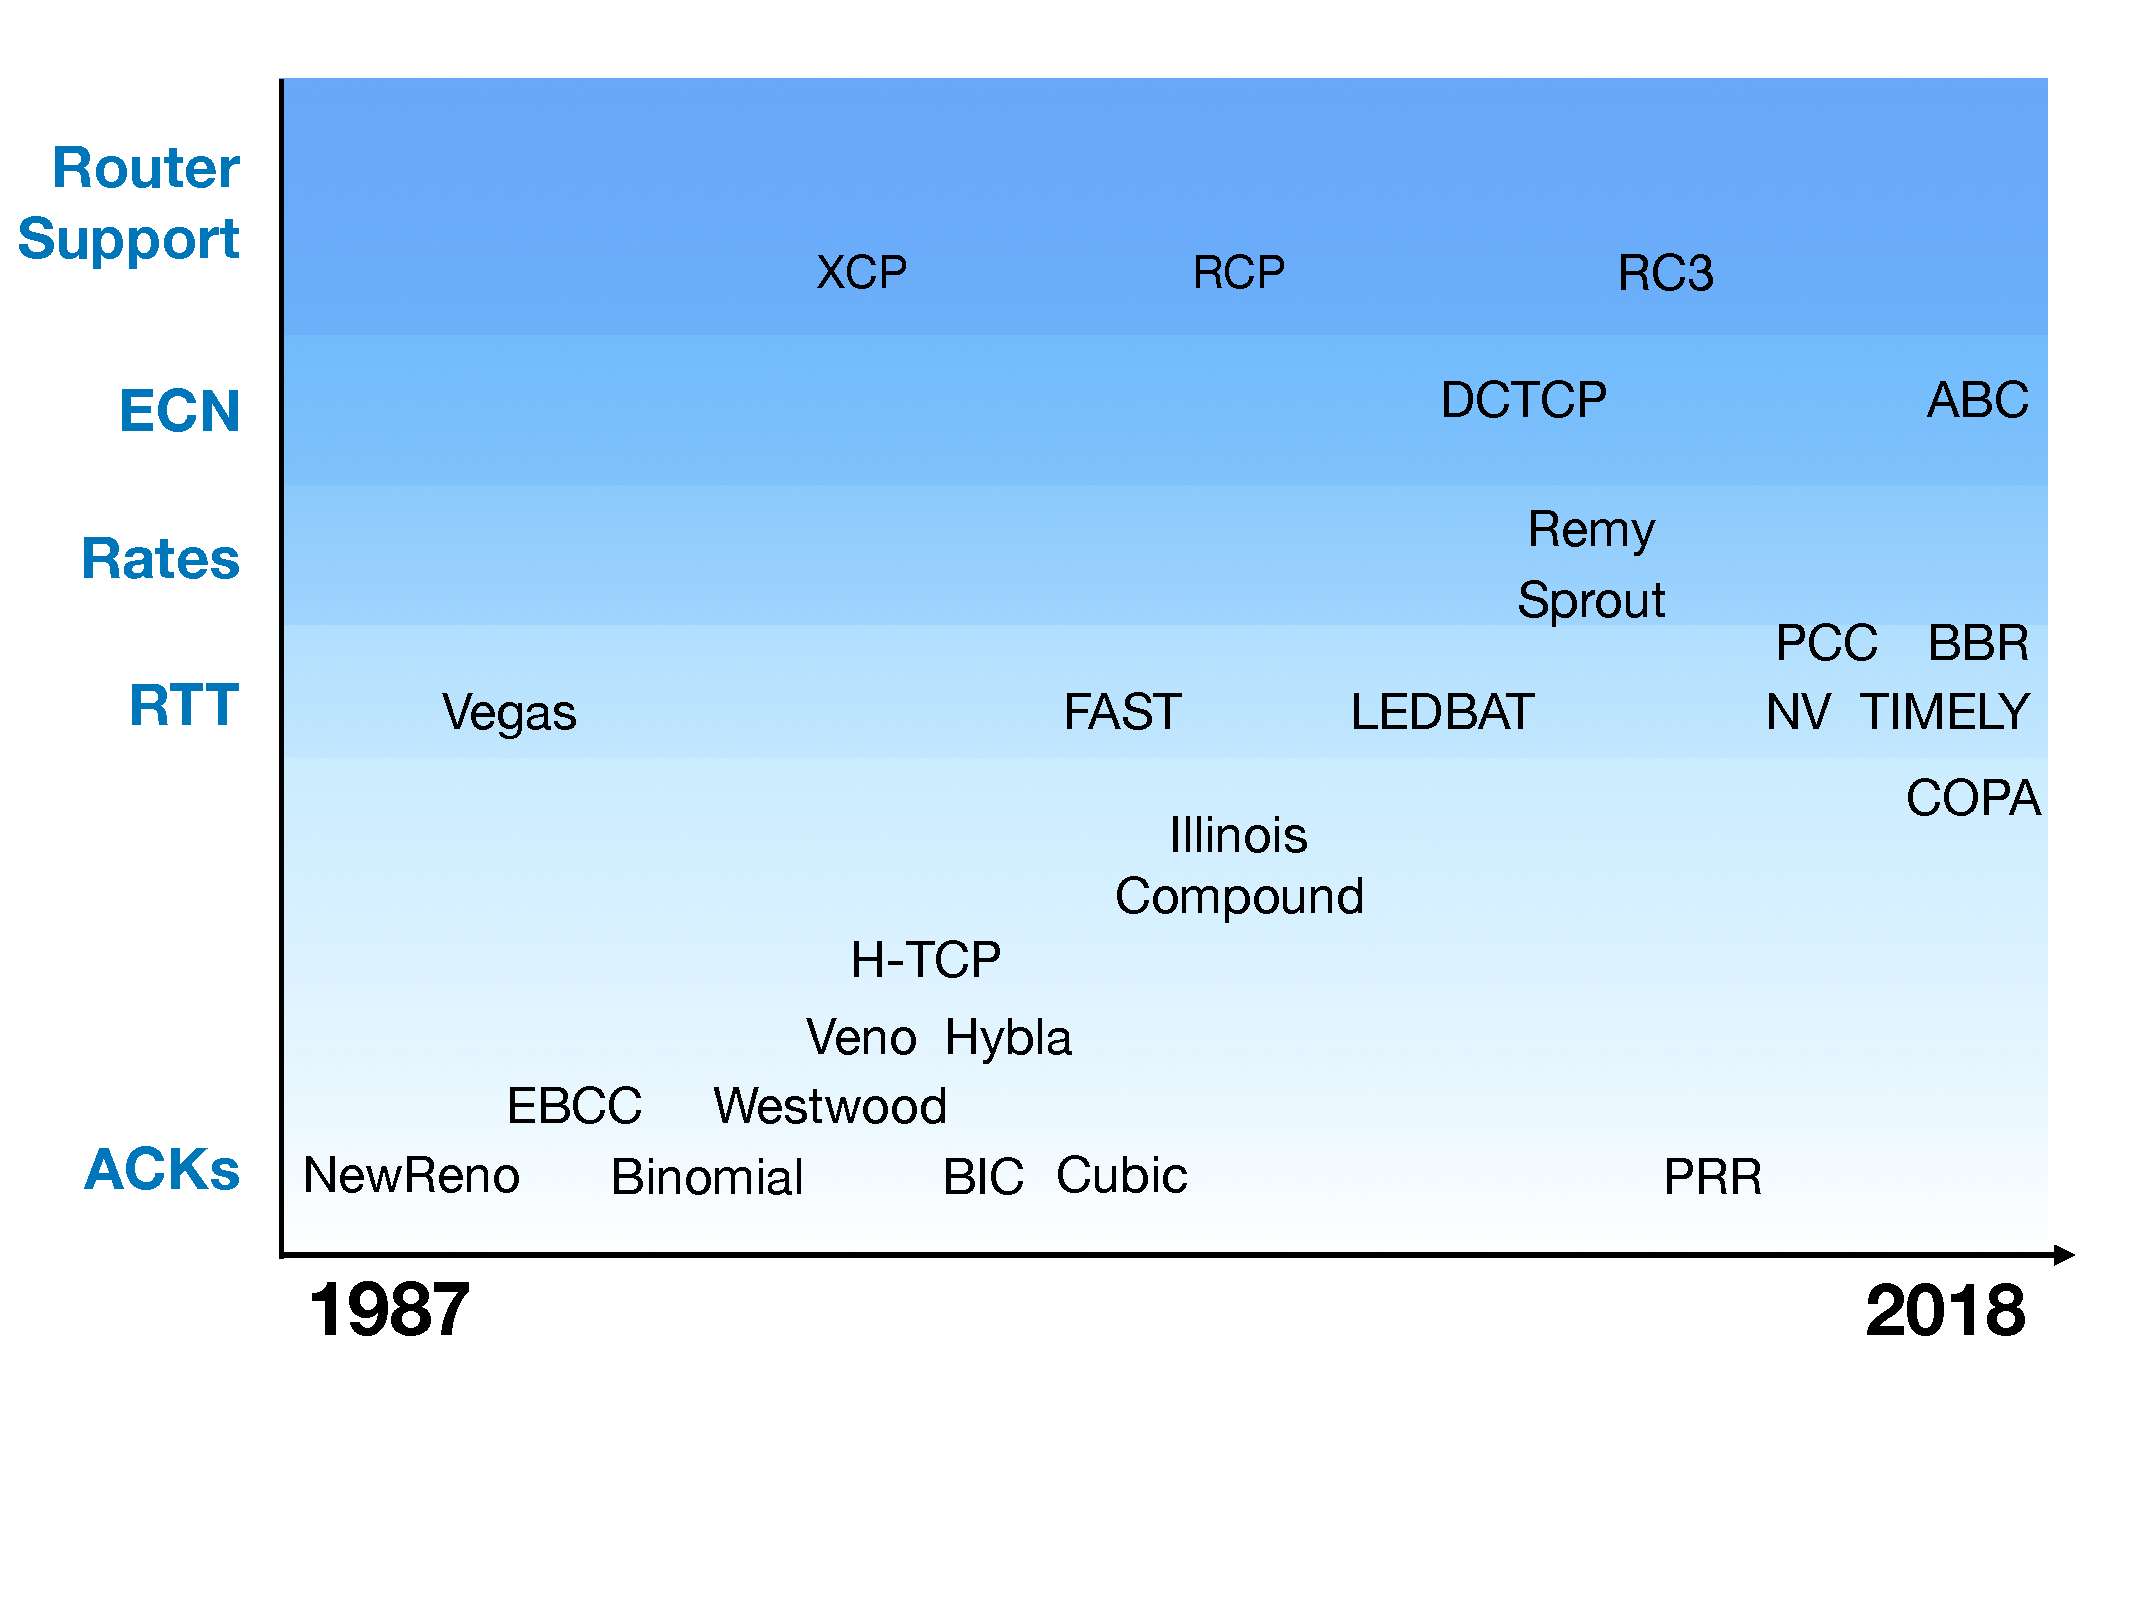
\includegraphics[width=\columnwidth]{img/cc-timeline}
    \vspace{-1cm}
    \caption{As link characteristics diversify, developers have developed a battery of congestion control algorithms, from the ``long-fat pipe'' schemes of the mid-2000s~\cite{westwood, veno, htcp, hybla} to purely delay-based~\cite{vegas, fasttcp, ledbat, nv, timely} and hybrid loss-delay~\cite{illinois, compound} schemes, and more recent proposals~\cite{pcc, remy, sprout, bbr, copa, abc}.}\label{fig:cctimeline}
\end{figure}

At its core, a congestion control protocol determines when each segment of data must be sent. Because a natural place to make this decision is within the transport layer, congestion control today is tightly woven into kernel TCP software and runs independently on each TCP connection.
However, this tight coupling is not fundamental to congestion control; rather,
it imposes an artificial restriction on algorithms to restrict their
computations to a single packet inter-arrival time lest they slow down the
flow.
%
Newly proposed algorithms lacking kernel implementations, such as
PCC~\cite{pcc}, Nimbus~\cite{nimbus}, Remy~\cite{remy}, and
Sprout~\cite{sprout}, all involve calculations that are cumbersome to perform in
the kernel, and are challenging to engineeer to meet tight performance
requirements.
%
For example, Nimbus uses Fast Fourier Transforms to determine the amount and
nature of the cross-traffic on the bottleneck link.

An operating system's TCP software is but one example of a {\em datapath}, the term we use for any module that provides data transmission and reception interfaces between higher-layer applications and lower-layer network hardware. Recently, many other datapaths have emerged, including user-space protocols atop UDP (e.g., QUIC~\cite{quic}, WebRTC~\cite{webrtc}, Mosh~\cite{mosh}), kernel-bypass methods (e.g., mTCP/DPDK~\cite{dpdk,mtcp,netmap}), RDMA~\cite{dcqcn}, multi-path TCP (MPTCP)~\cite{mptcp}, and specialized Network Interface Cards (``SmartNICs''~\cite{smartnic}). This trend suggests that the future will likely see many applications using datapaths different from kernel-supported TCP connections.

New datapaths typically do not offer much in terms of congestion control because implementing these algorithms correctly takes considerable time and effort. For instance, the set of available algorithms in mTCP~\cite{mtcp}, a TCP implementation on DPDK, is limited to a variant of Reno. Lest one dismiss this example as a case of a research project lacking in engineering resources, we note that QUIC, despite Google's imposing engineering resources, does not have most of the algorithms that have been implemented in the Linux kernel over many years.  We expect this situation to worsen with the emergence of new hardware accelerators and programmable network interface cards (NICs) because high-speed hardware designers tend to forego programming convenience for performance. The difficulty isn't the volume of code, but the many subtle correctness and performance issues in various algorithms that are tricky, requiring expertise to understand and resolve.

This paper starts from the observation, made in a recent position paper~\cite{ccp-hotnets}, that congestion control algorithms do not need to be implemented in the datapath. If the datapath encapsulated the information available to it about {\em congestion signals} like the round-trip time (RTT), packets received and lost, explicit congestion notification (ECN) markings, etc., and periodically provided this information via a well-defined interface to an off-datapath module, then congestion control algorithms could run in the context of that module. Then, by exposing an analogous interface to control transmission parameters such as the window size, pacing rate, and transmission pattern, the datapath could transmit data according to the policies of the off-datapath congestion control algorithm. 

Furthermore, an operating system's TCP software is but one example of a {\em
  datapath}, the term we use for any software that provides data transmission
and reception interfaces between applications and network hardware.
%
Recently, many datapaths other than the Linux kernel have emerged, including
user-space protocols atop UDP (e.g., QUIC~\cite{quic}, WebRTC~\cite{webrtc},
Mosh~\cite{mosh}), kernel-bypass methods (e.g.,
mTCP/DPDK~\cite{dpdk,mtcp,netmap}), RDMA~\cite{dcqcn}, multi-path TCP
(MPTCP)~\cite{mptcp}, and specialized Network Interface Cards
(``SmartNICs''~\cite{smartnic}).

The work described in this paper starts from the observation, first made in a
recent position paper~\cite{ccp-hotnets}, that congestion control algorithms do
not need to be implemented in the datapath. If the datapath encapsulated the
information available to it about {\em congestion signals} like the round-trip
time (RTT), packets received and lost, explicit congestion notification (ECN)
markings, \etc, and periodically provided this information via a well-defined
interface to an off-datapath module, then congestion control algorithms could
run in the context of that module.
%
If the datapath further exposes an interface to control transmission parameters
such as the window size or the pacing rate, the off-datapath congestion control
algorithm could instruct the datapath to transmit data according to its
policies.
%
Of course, the datapath (\eg Linux kernel TCP stack) must be modified to expose
such an interface, but such an effort only needs to be undertaken once for each
datapath, and does not grow with the number of congestion control algorithms.

We use the term {\em Congestion Control Plane (CCP)} to refer to this off-datapath module. Running congestion control in the CCP offers the following benefits:
\begin{enumerate}
    \item {\bf Higher ``velocity'' of development:} With the right abstractions,
      a congestion control designer can focus on the algorithmic essentials
      without worrying about the details and data structures of the
      datapath. The result is more expressive, easier to maintain code. We
      enable a deployment mode where CCP and the algorithm run at user level,
      implemented in the Rust language or using CCP's Python bindings. If the
      kernel module implementing CCP support is upstreamed, any new algorithms
      (including untrusted ones) can be deployed into high performance
      production systems over Linux without involving the upstreaming process.

    \item {\bf New capabilities:} CCP makes it easier to provide new
      capabilities, such as aggregate control of multiple flows as previously
      proposed in the congestion manager~\cite{cm}, and freedom from the ``ACK
      Clock'' for algorithms that require significant computation (e.g., signal
      processing, machine learning, \etc). All the benefits of a \userspace
      programming environment (libraries, debuggers, \etc) will be available to
      developers.

    \item {\bf Write-once, run-anywhere:} With CCP, developers can write a congestion control algorithm once and run it on any datapath that supports the specified interface. We focus on the Linux kernel datapath, but we have also implemented support for mTCP/DPDK and QUIC.
\end{enumerate}

\vspace{0.1in}
In summary, this paper contributes:

\begin{itemize}
\item A high-level event-driven language to specify congestion control
  algorithms. Algorithm developers specify congestion control behavior using
  combinations of events and conditions, such as the receipt of an
  acknowledgment or a loss event, along with corresponding handlers to perform
  simple computations directly in the datapath (\eg increment a window) or defer
  complex logic to a userspace component.

\item A specification of datapath responsibilities. These include congestion
  signals that a datapath should maintain (Table~\ref{tab:api}), as
  well as a simple framework to execute directives from a CCP program. This
  design enables ``write-once, run-anywhere'' protocols.

\item A preliminary demonstration of new capabilities enabled by CCP, including
  sophisticated new congestion control algorithms and the implementation of an
  aggregate congestion controller acting on behalf of multiple flows.

\item An evaluation of the fidelity of CCP relative to in-kernel
  implementations under a variety of link conditions. Our CCP implementation
  matches the performance of Linux kernel implementations at only a small
  overhead (5\% more CPU utilization in the worst case).
  %% Furthermore, we show it
  %% is feasible to implement infrequent congestion control even in low-RTT, high
  %% bandwidth environments.

\end{itemize}

\if 0
\begin{itemize}
\item A flexible API to request measurements from and exercise control over the datapath (\S\ref{sec:ccp}). We define a simple language with which algorithms can specify datapath congestion control behavior, including summaries over available measurement primitives and control decisions.

\item A specification of datapath responsibilities (\S\ref{s:datapath}). These include congestion signals that a datapath should maintain, as well as a simple framework to execute directives from a CCP program.
We describe our prototype implementation of CCP in Linux, comprising of a kernel module which uses the Pluggable TCP API and a user-space agent which runs and manages congestion control algorithms.
We have also prototyped CCP datapath implementations in QUIC and mTCP, but do not discuss them here.

\item An exploration of the design space of new capabilities enabled by CCP (\S\ref{s:capabilities}): the rapid development of new algorithms and implementing an aggregate congestion controller.

\item A demonstration of the fidelity of CCP in a variety of link conditions (\S\ref{sec:eval}). Our CCP implementation matches the performance of Linux kernel implementations at only a small overhead (5\% more CPU utilization in the worst case).

\end{itemize}
\fi

\section{Related Work}
\label{s:relwork}
%The CCP aims to provide a API for congestion control that decouples congestion control logic from the datapath, while keeping accurate measurement information from the datapath.

eBPF~\cite{ebpf} allows developers to define programs that can be safely executed in the Linux kernel. These programs can be attached to kernel functions and used for debugging. TCP BPF~\cite{tcpbpf} is an extension on top of BPF that allows customization of TCP connection settings, such as the TCP buffer size or SYN RTO, based on socket information such as IP address and port number. While it may be possible to develop a BPF backend to execute CCP fastpath programs, unlike \ct{libccp}, this method is not portable to other datapaths. Exploring BPF support in CCP remains future work.

Linux includes a pluggable TCP API~\cite{lwn-pluggable-tcp}, which exposes various statistics for every connection, including delay, rates averaged over the past RTT, ECN information, timeouts, and packet loss. 
icTCP~\cite{icTCP} is a modified TCP stack in the Linux kernel that allows user-space programs to modify specific TCP-related variables, such as the congestion window, slow start threshold, receive window size, and retransmission timeout. QUIC~\cite{quic} also offers pluggable congestion control. CCP extracts common primitives for congestion control across multiple datapaths, supporting off-datapath programmability with the performance of in-datapath implementations.

HotCocoa~\cite{hotcocoa} introduces a domain specific language to allow developers to compile congestion control algorithms directly into  programmable NICs to increase efficiency in packet processing. By contrast, CCP allows developers to write algorithms in user-space with the full benefit of libraries and conveniences such as  floating point operations (\eg for Fourier transforms). 
% in their congestion control algorithms traditionally not available in hardware. 
In addition, the congestion signals exposed by CCP datapaths are not tied to the ACK clock, allowing users to implement a wider class of algorithms. 

\if 0
The CCP API automatically supports ``write once, run everywhere'' behavior, so algorithms can instantly be run on various datapaths. CCP's fold functions also provides accurate per-packet calculations over congestion signals, and CCP methods run at kernel rates, even through the CCP runs in user-space.
\fi

Structured Streams~\cite{structuredstreams} is a datapath that proposes preventing head-of-line blocking by managing streams between the the same two hosts together, and applying a hereditary structure on streams. CCP does not change the underlying structure of the transport on the datapath; the Linux kernel datapath, for example, uses TCP streams. The congestion manager (CM~\cite{cm}) introduces an in-kernel agent to perform congestion control operations for a group of flows together. CCP is the first system to both provide flow aggregation capabilities \textit{and} an API for developers to develop novel algorithms, and it does so with few changes to the datapath.

There is a wide range of previous literature on moving kernel functionality into user-space. 
The Exokernel~\cite{exokernel} is an operating system architecture that securely
exports hardware functionality into untrusted user-space library operating systems.  
Arrakis~\cite{arrakis2014} is system that facilitates kernel-bypass networking for applications via SR-IOV. 
IX~\cite{ix} is a dataplane operating system that separates the management functionality of the kernel from packet processing. 
Alpine~\cite{alpine} moves all of IP and TCP layer into user-space.
Whereas these systems use hardware virtualization to allow applications to have finer grained control over their networking resources,
CCP exposes only congestion control information to user-space. 
Moreover, CCP is also agnostic to the datapath; datapaths for library operating systems could support the CCP API as well.
%Other systems aim to move the entire networking stack into userspace~\cite{thekkath,alpine}. 

\section{CCP Design Principles}
\label{s:design}
%
\begin{figure}[t]
\centering
    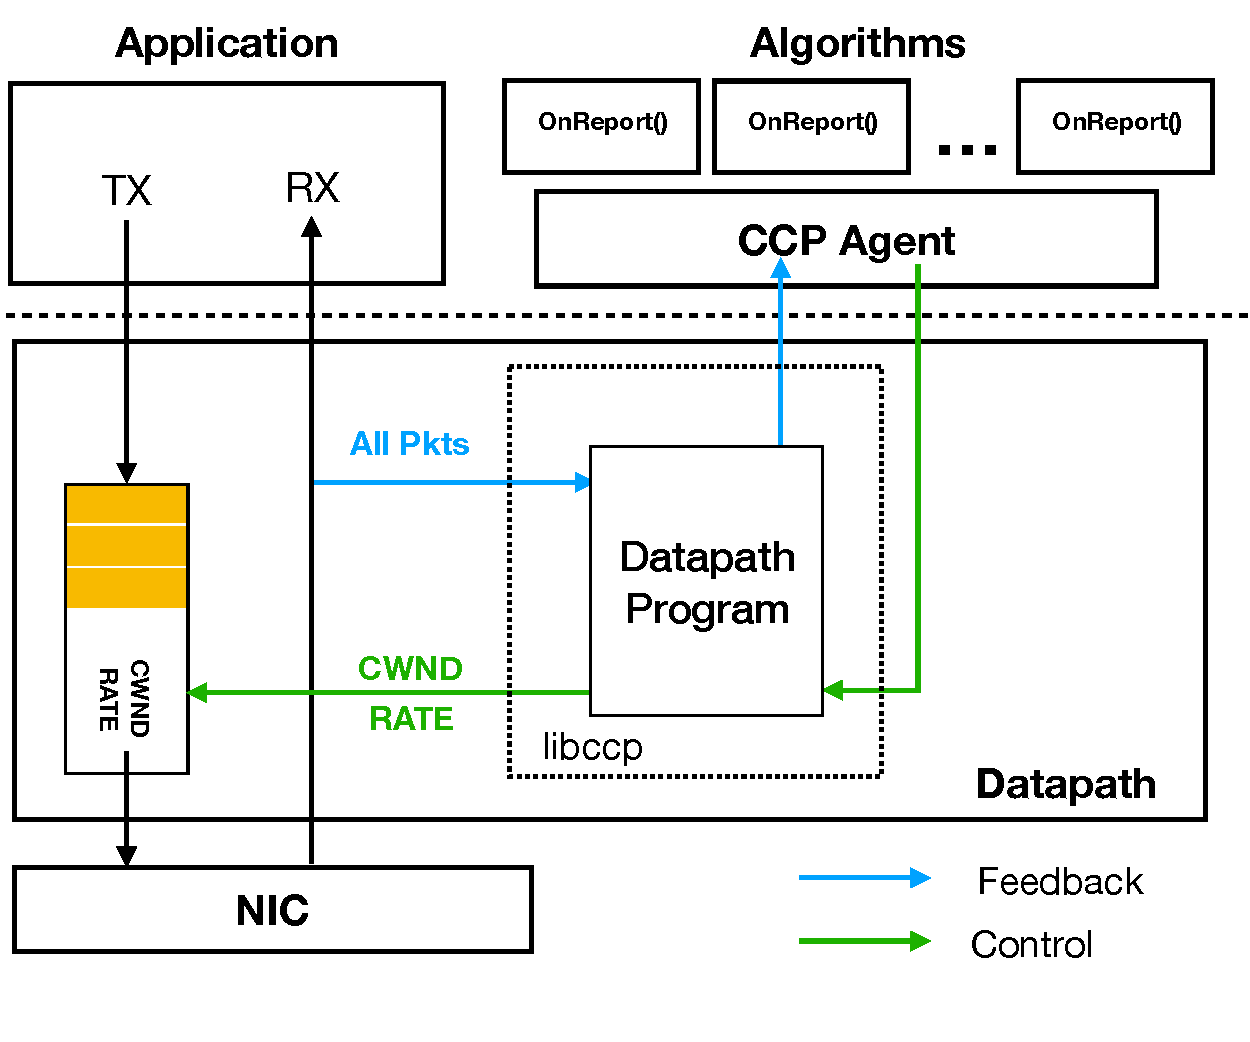
\includegraphics[width=\columnwidth]{img/ccp_design_sigcomm}
    \caption{Congestion control algorithms in CCP are distinct from the application and datapath.
    Users specify control patterns to set the congestion window or rate,
    and fold functions to define how to summarize datapath messages into reports processed in CCP.}\label{fig:design}
\end{figure}
%

To enable rich new congestion control algorithms on datapaths,
CCP must provide a low-barrier programming environment and access
to libraries (\eg for optimization, machine learning, \etc).
%
Further, new algorithms should also achieve high performance running at tens of
Gbit/s per connection with small packet delays in the datapath.

\subsection{CCP-Datapath Isolation}
\label{s:datapath:isolation}
Should congestion control algorithms run in the same address space as the
datapath? There are conflicting factors to consider:

\Para{Safety.} Supporting experimentation with algorithms and the possibility of
including \userspace library code means that programs implementing congestion
control algorithms should be considered untrusted. If algorithms and the
datapath are in the same address space, bugs in algorithm or library code could
cause datapath crashes or create vulnerabilities leading to privilege
escalations in the kernel datapath.

\Para{Performance.} Congestion control algorithms can access the datapath's
congestion measurements with low delays and high throughput if the two reside in
the same address space.

\Para{Flexibility.} We anticipate future use-cases of the CCP architecture where
a congestion control algorithm may run on a machine different from the sender,
enabling control policies across groups of hosts.

Our design restructures congestion control algorithms into two components in
separate address spaces: an off-datapath {\em CCP agent} and a component that
executes in the datapath itself.
%
The CCP agent provides a flexible execution environment for user-specified
congestion control algorithms, by receiving congestion signals from the datapath
and invoking the algorithm code on these signals.
%
The datapath component is responsible for processing feedback (\eg TCP or QUIC
ACKs, packet delays, \etc) from the network and the receiver, and provides
restricted aggregations over congestion signals for the algorithms running in
the CCP agent.
%
Further, the datapath component provides interfaces for the CCP agent to set
congestion windows and pacing rates.

An alternative design in the case of the kernel datapath, which is to allow
fully functional kernel modules with software fault isolation (\eg
LXFI~\cite{lxfi}) from the rest of the kernel, will likely involve significant
performance impediments.\footnote{Further, an approach such as LXFI also
  requires a careful annotation of kernel functions, and the specification of
  principals and kernel API integrity rules---a challenging task because the
  network stack has a large number of functions with subtle behaviors.}
%
Instead, our fast path programs are written in a restrictive domain-specific language (\Sec{sec:ccp})
that is free from broad classes of vulnerabilities.\footnote{Note that while \texttt{libccp}, our fast path library (\Sec{s:datapath:libccp}), enforces runtime safety of fast-path algorithm logic,
algorithm implementations are nevertheless free to set arbitrary rates or congestion windows.
As any application can open UDP sockets and congest the network, we do not restrict this behavior.}
Meanwhile, slow path programs have full access to the \userspace programming environment,
tools, and libraries.

%% Explicit CCP and datapath separation also enables future use cases where
%% congestion control algorithms may run on a machine different from the sender to
%% centralize congestion control policies across groups of hosts.

%% rephrase the stuff below
Our design supports both modes, but we focus on how to achieve high performance
and fidelity when CCP is in a different address space, including the important
case when the datapath is kernel TCP and CCP is in user space.

\begin{table}[]
    \centering
    \begin{tabular}{c|c|c}
        Implementation & Reporting Interval & Mean Throughput \\
        \hline
        Kernel & - & $43$ Gbit/s \\
        CCP & Per ACK & $29$ Gbit/s \\
        CCP & Per $10$ ms & $41$ Gbit/s \\
    \end{tabular}
    \caption{Single-flow throughput for different reporting intervals between
      the Linux kernel and CCP \userspace, compared to kernel TCP
      throughput. Per-ACK feedback (0 $\mu$s interval) reduces throughput by
      32\% while using a $10$ ms reporting interval
      achieves almost identical throughput to the kernel. Results as the number
      of flows  increases are in
      \S\ref{sec:eval:whyfold}.}\label{tab:perf:interval}
\end{table}

\subsection{Decoupling congestion control from the ACK clock}

Typical congestion control
implementations in the Linux kernel are coupled to the so-called ``ACK-clock,''
\ie algorithm functionality is invoked upon receiving a packet acknowledgment in
the networking stack.
%
While this is also true of a CCP algorithm's fast path, the CCP slow path is
only invoked when the user specifies, whether less frequently than per-ACK or in response to certain urgent conditions.
%
To support this, CCP exposes a \ct{report} instruction for fast path programs to send a
report of the most recent user-defined measurement state in the kernel to the slow path.

This decoupling of algorithm logic from the ACK clock has two benefits.
%
First, the user can develop congestion control algorithms free from the strict
time restrictions rooted in the inter-arrival time of packet acknowledgments,
especially at high link rates.
Hence, users can implement algorithms that use complex logic and yet retain high performance.

Second, providing per-ACK notifications from the kernel to \userspace would incur
significant overhead.
%
Table~\ref{tab:perf:interval} shows that for a single saturating \ct{iperf}
connection over a loopback interface, Linux kernel TCP on a server machine
with four 2.8-Ghz cores achieves $45$ Gbit/s running Reno.
%
In comparison, per-ACK reporting from the kernel to the CCP \userspace achieves
only 68\% of the kernel's throughput.
%
By increasing the time between reports sent to the slow path to 10 ms (see the
``per 10 ms'' row), CCP Reno achieves close to the kernel's throughput.

Given that CCP should report measurements only infrequently, a key question is
how best to summarize congestion signals within the fast path, so that CCP
algorithms can achieve high fidelity compared to a baseline that implements the
algorithm completely within the kernel.
Although we are optimistic that a good design can achieve high fidelity because the natural time-scale for end-to-end
congestion control is the RTT between sender and receiver,
achieving it requires a careful design of the information channel between the kernel and CCP \userspace.
Indeed, in \S\ref{sec:eval:fidelity} we show that using a
larger reporting period does not affect the fidelity of CCP algorithm
implementations relative to native in-kernel implementations.


\subsection{Exercising Control over Datapath Functions}
\ngs{content below requires some deduplication with section that follows}

% CCP algorithms specify datapath behavior using two mechanisms: {\em fold functions} and {\em control patterns},  whose directives are used by the datapath to summarize congestion signals sent to CCP, and {\em send patterns}, which control packet transmissions on the datapath. 
 
Congestion-control algorithms written in CCP are not tied to the traditional ``ACK clock'', but rather operate on summaries that encapsulate observations over multiple ACKs received by the datapath sender.
CCP algorithms specify datapath behavior using two mechanisms: {\em fold functions} and {\em control patterns}, whose directives are interpreted by the datapath to summarize congestion signals sent to CCP and control packet transmissions on the datapath, respectively. 
 
\paragrapha{Congestion signals and fold functions} All CCP-compatible datapaths should export a well-defined set of congestion signals (Table~\ref{tab:datapath:signals}). There are two kinds of congestion signals: \texttt{Ack} signals, which are computed directly on each ACK (e.g., bytes acked in order, bytes acked out of order, RTT sample, etc.) and \texttt{Flow} signals, which are statistics maintained for the flow (e.g., outgoing and incoming rates). Most of these signals are updated on the arrival of an ACK; the exceptions are: \texttt{was\_timeout} and \texttt{lost\_pkts\_sample} updated on a timeout; and \texttt{bytes\_in\_flight} and \texttt{packets\_in\_flight} updated on packet transmissions.
 
% update others might update on a timeout or at other times. \ma{this is
% vague. what `other times'?}

CCP may read but not write these signals. The only way to gain access to them is via a fold function, which specifies how the datapath should summarize the congestion signals in a single reporting period. 
%For example, a CCP algorithm may ask to receive the sum of the bytes acknowledged in order, the moving average of the RTT samples, and the latest value of the flow's outgoing rate in a reporting period. 
 
%CCP is unaware of how a datapath computes these signals; for example, it does not know which variables the datapath uses to compute the signals. A CCP algorithm, however, specifies how it wants the datapath to summarize each signal over a reporting period using a small language. 
 
%

Fold functions express simple operations over the congestion signal primitives. Table~\ref{tab:datapath:operators} contains the operations each datapath should be able to compute. A CCP algorithm expresses fold functions in a small, restrictive domain-specific language. Each datapath must support this language. For software datapaths, we have developed \texttt{libccp}, a library that provides a reference implementation of fold function computations in this language and other features common to all datapaths (see \S\ref{s:datapath:libccp}). 
 
The fold function defines a structure called \texttt{Summary}. This structure is maintained by the datapath and encapsulates all measurements reported to CCP by the datapath. The CCP algorithm specifies the fields of the \texttt{Summary} structure in the fold function and how to compute each field from congestion signals. The algorithm may define as many fields as it wants in the \texttt{Summary} structure. The datapath writes the values of these fields using the logic supplied by the CCP algorithm.
 
The following fold function shows an example of how to request the number of bytes delivered in order within the reporting period. The sender's datapath runs this function on each received ACK, \texttt{A}:
 
\begin{minted}{lisp}
  (def (Summary.acked 0))
  (:= Summary.acked
    (+ Summary.acked A.bytes_acked))
\end{minted}
 
%The fold function defines a \texttt{Summary} signal, which is the third type of signal maintained by the datapath. 
%Unlike \texttt{Ack} and \texttt{Flow} signals, which are read-only, \texttt{Summary} signals are writeable by the CCP algorithm. 
 
In the example above, the fold function defines a field, \texttt{Summary.acked}, and specifies that on each invocation (typically every received ACK), it should be incremented by the number of in-order bytes observed since the last invocation. After delivering the summary, the datapath resets each reported \texttt{Summary} field to the specified initial value.
 
%We specify the complete list of available signals and built-in operations on them in \S\ref{s:datapath:fold}.
 
\paragrapha{Control patterns} CCP algorithms can specify the congestion window or pacing rate using simple functions supported by the datapath. These can be set to either absolute values or relative to current values. The algorithms can also specify timing patterns according to which summary reports from fold functions and window/rate settings are executed by the datapath. 
The ability to specify timing patterns is useful for two reasons. First, algorithms may wish to specify patterns of sending; BBR~\cite{bbr}, for example, sends pulses of different magnitudes for specific time durations. Second, algorithms may wish to specify the precise intervals over which congestion signals should be gathered and reported (e.g., once every half-RTT).
 
\begin{minted}{rust}
SetCwndAbs(...) => WaitRtts(0.5) => Report()
\end{minted}
 
Control patterns use \texttt{=>} to specify that the directive on the right should happen after the one on the left. This example pattern uses the \texttt{WaitRtts()} directive to specify that the datapath should set the congestion window to the specified value, wait for a half-RTT, and then report a summary to CCP. After this report, the pattern will reset Summary state and loop back to \texttt{SetCwndAbs()}.
 
%We study this behavior with several experiments in \S\ref{s:eval:fidelity}.
 
Figure~\ref{fig:design} shows the architecture of a CCP-enabled sender, highlighting how the components we have discussed in this section fit together. 



\subsection{Alternative Designs}
\label{sec:design:alternatives}

\an{eBPF is limited and pluggable tcp is strictly less general than us.}

\an{address congestion manager here}



\section{Writing Algorithms in CCP}
%
\begin{figure}[t]
\centering
    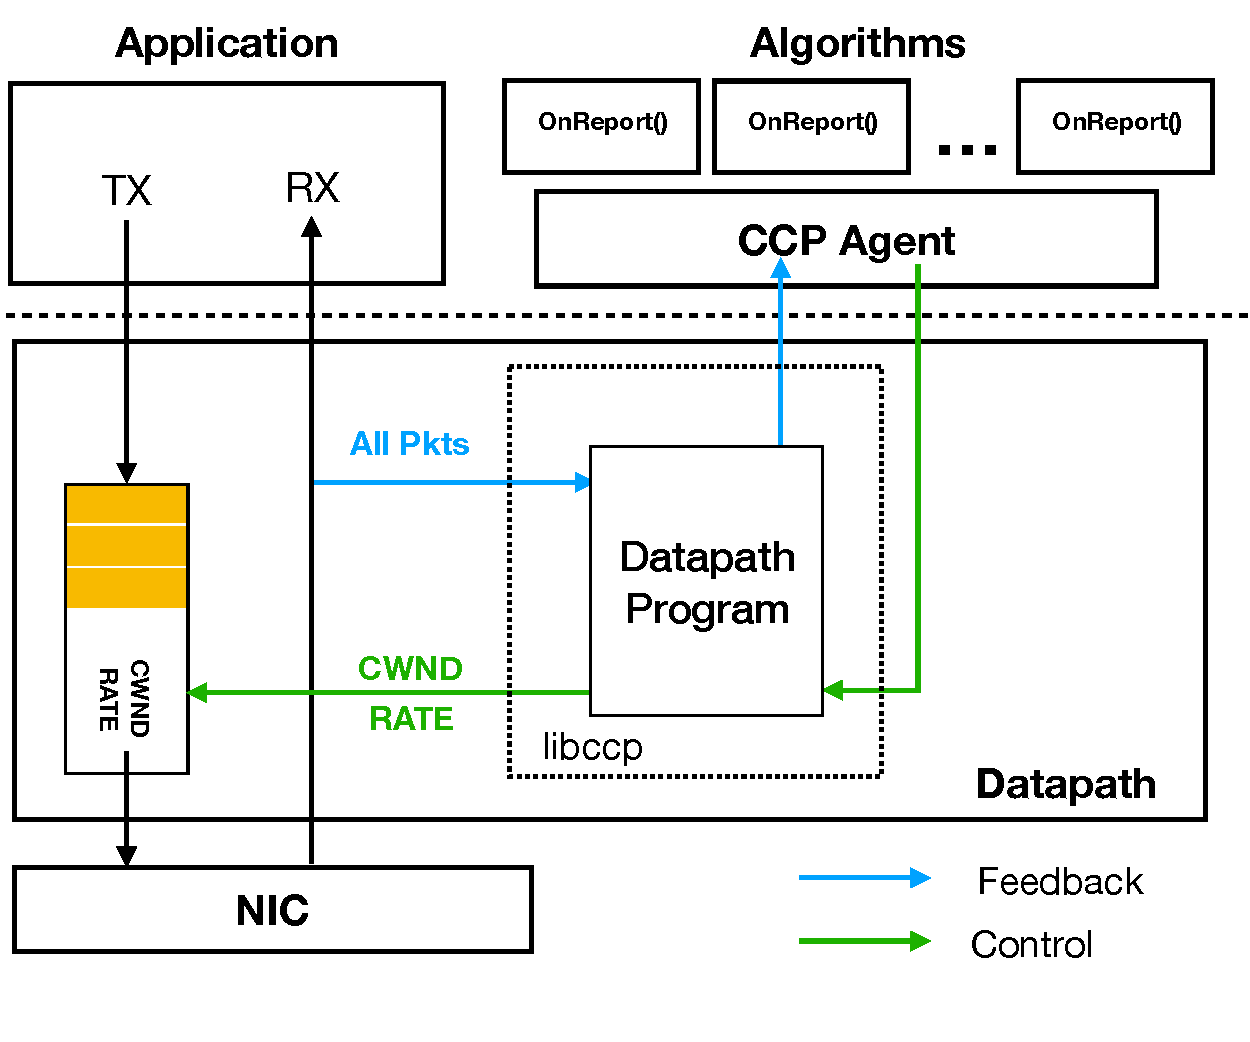
\includegraphics[width=\columnwidth]{img/ccp_design_sigcomm}
    \caption{Congestion control algorithms in CCP are distinct from the application and datapath.
    Users specify an \texttt{onCreate()} handler which CCP calls when a new flow begins. 
    In this handler, algorithms install (1) a datapath program. 
    This datapath program aggregates incoming measurements (2) using user-defined fold functions and occasionally sends reports (3) to CCP, which calls the \texttt{onReport()} handler.
    The \texttt{onReport()} handler can update (4) the datapath program, which uses its defined control patterns to enforce (5) a congestion window or pacing rate.
    }\label{fig:design}
\end{figure}
%
\label{sec:ccp}
\begin{table}
    \centering
    \footnotesize
    \begin{tabular}{@{} p{0.35\columnwidth}p{0.5\columnwidth}}
        \hline
        \hline
        \multicolumn{2}{c}{Primitive congestion signals} \\
        \hline
        \hline
        \textbf{Signal} & \textbf{Definition} \\
        \texttt{Ack.bytes\_acked}, \texttt{Ack.packets\_acked} & In-order acknowledged \\
        \texttt{Ack.bytes\_misordered}, \texttt{Ack.packets\_misordered} & Out-of-order acknowledged \\
        \texttt{Ack.ecn\_bytes}, \texttt{Ack.ecn\_packets} & ECN-marked \\
        \texttt{Ack.lost\_pkts\_sample} & Number of lost packets \\
        \texttt{Ack.now} & Datapath time (e.g., Linux \texttt{jiffies})\\
        \texttt{Flow.was\_timeout} & Did a timeout occur? \\
        \texttt{Flow.rtt\_sample\_us} & A recent sample RTT \\
        \texttt{Flow.rate\_outgoing} & Outgoing sending rate \\
        \texttt{Flow.rate\_incoming} & Receiver-side receiving rate  \\
        \texttt{Flow.bytes\_in\_flight}, \texttt{Flow.packets\_in\_flight} & Sent but not yet acknowledged \\
        & \\
        \hline
        \hline
        \multicolumn{2}{c}{Operators} \\
        \hline
        \hline
        \textbf{Class} & \textbf{Operations} \\
        Arithmetic & \texttt{+}, \texttt{-}, \texttt{*}, \texttt{~/} \\
        Assignment & \texttt{:=} \\
        Comparison & \texttt{==}, \texttt{<}, \texttt{>}, \texttt{or}, \texttt{and} \\
        Conditionals & \texttt{If} (branching) \\
        & \\
        \hline
        \hline
        \multicolumn{2}{c}{Variable Scopes} \\
        \hline
        \hline
        \textbf{Scope} & \textbf{Description} \\
        \texttt{Ack} & Signals measured per packet \\
        \texttt{Flow} & Signals measured per connection \\
        %% \texttt{Control} & Never reset except by \texttt{update\_fields()} in user-space \\
        %% \texttt{Report} & Maintained until a call to \texttt{(report)}, then reset to defaults \\
        \texttt{Timer} & Multi-resolution timer that can be zeroed by a call to \ct{reset} \\
    \end{tabular}
    %\vspace{0.075in}
    \caption{Datapath language: congestion signals, operators, and scopes.}\label{tab:api}
\end{table}

Figure~\ref{fig:design} shows the control loop of a congestion control algorithm in CCP.
Users implement two callback handlers (\ct{onCreate()} and \ct{onReport()}) in the CCP agent
and one or more datapath programs.
When a new flow is created, CCP's datapath component invokes the \ct{onCreate()} handler.
The implementation of \ct{onCreate()} must install an initial datapath program for that flow.
%
Datapath programs could compute summaries over per-packet
congestion signals (such as a minimum packet delay or a moving average of packet
delivery rate) and report summaries or high priority conditions
(such as loss) to the CCP agent.
On a report, the CCP agent invokes the \ct{onReport()} handler
which contains the bulk of the logic of the congestion control algorithm.
The \ct{onReport()} function computes and installs the flow's congestion
window or sending rate using the signals from the datapath report.
It may also replace the datapath program entirely with different logic.

\subsection{Datapath Program Abstractions}
\label{s:ccp:datapath_programs}
CCP's datapath programs are written in a simple domain specific language.
These programs exist in order to provide a per ACK execution environment, where algorithms can define and update variables per ACK and perform \textit{control actions}, in response to the values of these variables.

Figure~\ref{lst:design:simple_datapath_prog} shows a program that counts the cumulative number of packets acknowledged and lost and reports these counters immediately upon a loss.
\begin{figure}[t]
{\footnotesize
\begin{minted}[xleftmargin=\parindent,linenos]{lisp}
(def (Report (volatile acked 0) (volatile lost 0)))
(when true
  (:= Report.acked (+ Report.acked Ack.bytes_acked))
  (:= Report.lost  (+ Report.lost  Ack.lost_pkts_sample))
  (fallthrough))
(when (> Report.lost 0) (report))
\end{minted}
\caption{A simple datapath program to count bytes acked and report on losses.} \label{lst:design:simple_datapath_prog}
}
\end{figure}
The first statement of the program allows users to define custom variables.
The ``Report'' block signifies that these variables should be included in the report message sent to the CCP agent.
The \ct{volatile} marker means that these variables should be reset to their initial values, 0, after every report to the CCP agent.

Following the \texttt{def} block, \textit{fold functions} provide custom summaries over primitive congestion signals.
Datapath programs have read access to these \textit{primitive congestion signals} (prefixed with ``Ack.'' or ``Flow.'' to specify their measurement period), which are exposed by the datapath on every incoming packet. Such signals include the round trip delay sample, the number of bytes the datapath believes have been dropped by the network, and the delivery rates of packets. Table ~\ref{tab:api} enumerates the primitive congestion signals we support.
Users can write simple mathematical summaries over these primitive signals, as shown in Lines 3-4 of Figure~\ref{lst:design:simple_datapath_prog}.

Finally, algorithms can perform control actions in response to conditions defined by the fold function variables, \eg updating a rate or cwnd or reporting the user defined variables to the CCP agent.
As shown in Figure~\ref{lst:design:simple_datapath_prog}, the program defines a series of \ct{when} clauses, and performs the following block only if the condition was evaluated to true.

CCP's datapath program language provides an event driven programming model.
\ct{(when true...)} signifies that the body should be evaluated on every packet.
This is where the program might calculate fold function summaries.
\ct{when} clauses also have access to all the fold function variables, as well as timing related counters.
The \ct{report} instruction causes the datapath to transmit the \ct{acked} and \ct{lost} counters to the CCP agent.
By default, the program evaluates until one \ct{when} clause evaluates to true; the \ct{(fallthrough)} instruction at the end of the first \ct{when} indicates that susbequent \ct{when} clauses should also be evaluated.

%  CCP's datapath programs are written in a restrictive
% domain-specific language.
% Conceptually, datapath programs contain state initializations, \ie a \ct{def}
% clause, and event specifications, \ie a series of \ct{when} clauses.
% The datapath checks event conditions on every incoming packet and timeout event.
% If an event condition evaluates to true, the body of the \ct{when} clause is executed as the corresponding
% action.
% For example, the following program counts the cumulative
% number of packets acknowledged and lost, and it reports these counters immediately upon a loss:

% {\footnotesize
% \begin{minted}
% {lisp}
% (def (Report (volatile acked 0) (volatile lost 0)))
% (when true
%   (:= Report.acked (+ Report.acked Ack.bytes_acked))
%   (:= Report.lost  (+ Report.lost  Ack.lost_pkts_sample))
%   (fallthrough))
% (when (> Report.lost 0) (report))
% \end{minted}
% }

% Here, \texttt{(when true ...)} signifies that the body should be evaluated on every packet.
% Correspondingly, \texttt{(fallthrough)} indicates that subsequent \texttt{when} clauses should be evaluated.
% The \ct{report} instruction causes the datapath to
% transmit the \ct{acked} and \ct{lost} byte counters to the slow path whenever
% the \ct{lost} counter becomes greater than zero.
% Since \ct{acked} and \ct{lost} are marked \ct{volatile}, these values are reset to their initial value, 0, 
% after every call to \ct{report}.

% Datapath programs have read access to {\em primitive congestion signals} 
% (prefixed with ``\ct{Ack.}'' or ``\ct{Flow.}'' to specify their measurement period) that are
% exposed by the datapath on every incoming packet.
% Such signals include statistics such as the round trip delay sample obtained
% from the packet, the number of bytes that the stack believes have been dropped
% by the network, the delivery rate of packets at the receiver, and so on.
% Table~\ref{tab:api} enumerates the primitive congestion signals we support.

\subsection{CCP Algorithm Logic}
\label{s:ccp:ccp_algorithm_logic}
The \ct{onReport()} handler provides a way to
implement congestion control actions in \userspace in reaction to reports from the datapath.
For example, a simple additive-increase
multiplicative-decrease (AIMD) algorithm could be implemented in Python\footnote{Our CCP implementation is in Rust and exposes Python bindings (\S\ref{s:datapath}).} using
the \ct{acked} and \ct{lost} bytes reported every round-trip time from the datapath:

{\footnotesize
\begin{minted}{python}
def onReport(self, report):
  if report["lost"] > 0:
     self.cwnd = self.cwnd / 2
  else:
     acked = report["acked"]
     self.cwnd = self.cwnd + acked*MSS/self.cwnd
  self.update("cwnd", self.cwnd/MSS)
\end{minted}
}

We have implemented complex functionality within congestion control algorithms
by leveraging slow-path logic, for example, a congestion control
algorithm that uses Fast Fourier Transform (FFT) operations~\cite{nimbus}.

If the round-trip time of the network is a few milliseconds or more,
it is possible to locate congestion control algorithm logic entirely within CCP
with high fidelity relative to a per-packet update algorithm, as we show in \S\ref{sec:eval:fidelity}.

\subsection{Example: BBR}
\label{s:ccp:bbr}
As a more involved example, we show below how various components of TCP BBR~\cite{bbr} are implemented using the CCP API.
A BBR sender estimates the rate of packets delivered to the receiver, and 
sets its sending rate to the maximum delivered rate (over a sliding time window), 
which is believed to be the rate of the bottleneck link between the sender and the receiver.

This filter over the received rate is expressed simply in a fold function:
{\footnotesize
\begin{minted}{lisp}
(when true
    (:= minrtt (min minrtt Ack.rtt_sample_us))
    (:= curr_btl_est (max curr_btl_est Flow.rate_incoming))
    (fallthrough))
\end{minted}
}

To determine whether a connection can send more than its current sending rate,
BBR probes for additional available bandwidth by temporarily increasing its
sending rate by a factor (1.25$\times$) of its current sending rate.
%
To drain a queue that may have been created in the process, it also reduces its
rate by a reciprocal factor (0.75$\times$) before starting to send at the new estimated
bottleneck link rate.

The following excerpt expresses this sending pattern (for simplicity, we show only 2 transitions):
{\footnotesize
\begin{minted}{lisp}
(when (== pulseState 0)
  (:= Rate (* 1.25 curr_btl_est))
  (:= pulseState 1))
(when (&& (== pulseState 1) 
          (> Timer.micros Flow.rtt_sample_us))
  (:= Rate (* 0.75 curr_btl_est))
  (:= pulseState 2))
\end{minted}
}

Here, the variable \ct{pulseState} denotes the state of the sender's
bandwidth probing: probing with high sending rate (0) and draining queues with low
sending rate (1).
Each \texttt{when} clause represents a pulse state transition and is conditioned on the
resettable timer \texttt{Timer.micros}.
Upon the transition, the handler sets the \texttt{Rate} and advances \texttt{pulseState}.
After the last phase of the pulse, the handler would reset the timer and \ct{pulseState} to restart the sending pattern (not shown).
%\ma{is this too complicated to show? it would be nice to show a complete example.}

Figure~\ref{fig:ccp:bbr} shows
the impact of BBR's bandwidth probing\footnote{We only implement BBR's PROBE\_BW and PROBE\_RTT. Our implementation is here: \url{github.com/ccp-project/bbr}.} on the
achieved goodput and queueing delays when a single flow runs over a 48 Mbit/s
bottleneck link with a 20 ms round trip propagation delay.
%
BBR's windowed min/max operations and the RTT probing phase (showing steep rate
dips every 10 seconds) are implemented in the slow path's \ct{onReport()}
handler by installing a new fold function.
%
CCP's split programming model enables this flexible partitioning of functionality.

\begin{figure}[t]
\centering
    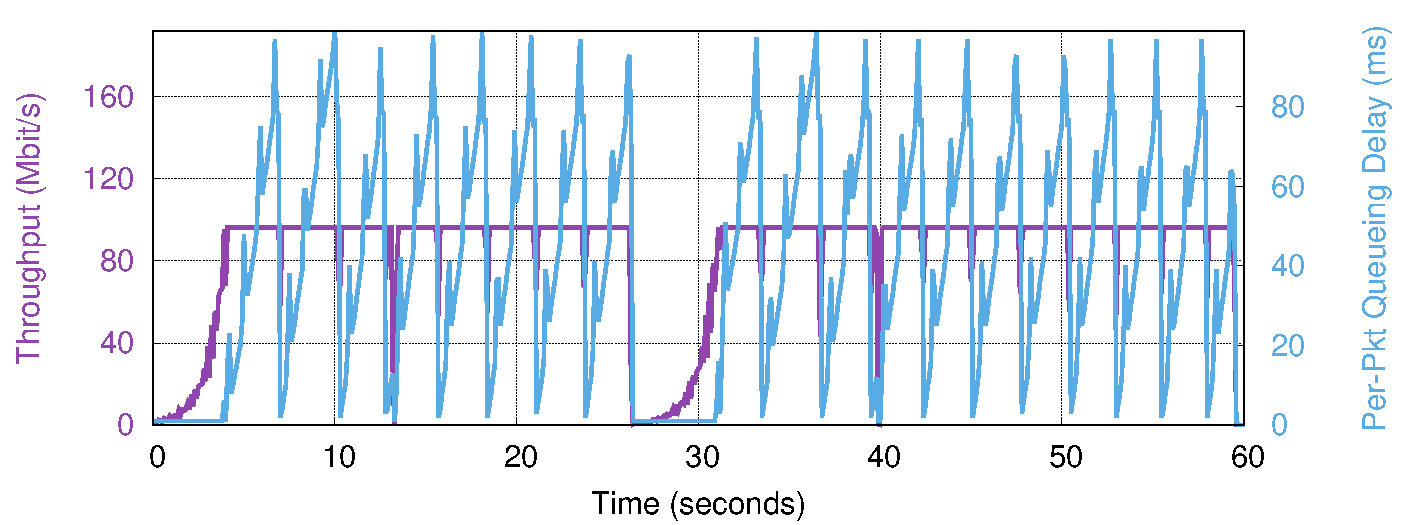
\includegraphics[width=\columnwidth]{img/bbr}
    \caption{
    Our CCP implementation of BBR used for a bulk transfer over a 48 Mbit/s link with a 20 ms RTT and 2 BDPs of buffering. The bandwidth probe phase can be seen in the oscillation of the queueing delay, and the RTT probe phase can be seen in the periodic dips in throughput.
    }\label{fig:ccp:bbr}
\end{figure}

\subsection{Case Study: Slow Start}
\label{s:ccp:ss}

Because algorithms no longer make decisions upon every ACK, CCP changes the way in which developers should think about congestion control, and correspondingly provides multiple implementation choices. As a result, new issues arise about where to place algorithm functionality. We discuss the involved trade-offs with an illustrative example: slow start.

Slow start is a widely used congestion control module in which a connection probes for bandwidth by multiplicatively increasing its congestion window (\texttt{cwnd}) every RTT. Most implementations increment \texttt{cwnd} per ACK, either by the number of bytes acknowledged in the ACK, or by 1 MSS. One way to implement slow start is to retain the logic entirely in CCP, and measure the size of the required window update from datapath reports. We show an example in Figure~\ref{lst:ccp:ss}. This implementation strategy is semantically closest in behavior to native datapath implementations.

\begin{figure}[t]
{\footnotesize
\begin{minted}{rust}
fn create(...) {
  datapath.install("
  (def (Report (volatile acked 0) (volatile loss 0)))
  (when true 
    (:= Report.acked (+ Report.acked Ack.bytes_acked)))
  (when (> Micros Flow.rtt_sample_us) (report) (reset))");
}
fn onReport(...) {
  if report.get_field("Report.loss") == 0 {
    let acked = report.get_field("Report.acked");
    self.cwnd += acked;
    datapath.update_field(&[("Cwnd", self.cwnd)]);
  } else { /* exit slow start */ }
}
\end{minted}
}
\vspace{-10pt}
\caption{A CCP implementation of slow start.} \label{lst:ccp:ss}
\vspace{-15pt}
\end{figure}

\begin{figure}
    \centering
    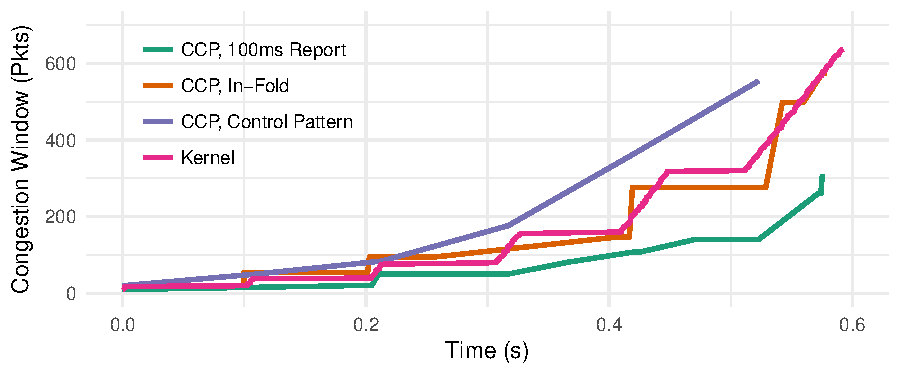
\includegraphics[width=\columnwidth]{img/ss-evo}
    \caption{Different implementations of slow start have different window update characteristics. The control pattern implementation is rate-based, so we show the congestion window corresponding to the achieved throughput over each RTT.}
    \label{fig:ccp:ss}
\end{figure}

For some workloads this approach may prove problematic, depending on the parameters of the algorithm. If the reporting period defined is large, then infrequent slow start updates can cause connections to lose throughput.
Figure~\ref{fig:ccp:ss} demonstrates that, on a $48$ Mbps, $100$ ms RTT link, different implementations of slow start exhibit differing window updates relative to the Linux kernel baseline.
A version with a 1-RTT reporting period lags behind the native datapath implementation. It is also possible to implement slow start within the datapath either by using congestion window increase (Figure~\ref{lst:ccp:ssfold}), or by using rate based control: 

{\footnotesize
\begin{minted}{lisp}
(when (> Timer.Micros Flow.rtt_sample_us)
    (:= Rate (* Rate 2))
    (:= Timer.Micros 0))
\end{minted}
}

\paragrapha{Take-away} As outlined in \S\ref{s:design}, the programming model of datapath programs is deliberately limited.
First, we envision that in the future, CCP will support low-level hardware datapaths---the simpler the fold function execution environment is, the easier these hardware implementations will be. Second, algorithms able to make complex decisions on longer time-scales will naturally do so to preserve cycles for the application and datapath; as a result, complex logic inside the fold function may not be desirable.

More broadly, developers may choose among various points in the algorithm design space. 
On one extreme, algorithms may be implemented almost entirely in CCP, using the fold function as a simple measurement query language.
On the other extreme, CCP algorithms may merely specify transitions between in-datapath fold functions implementing the primary control logic of the algorithm.
Ultimately, users are able to choose the algorithm implementation best suited to their congestion control logic and application needs.

\begin{figure}[t]
{\footnotesize
\begin{minted}{rust}
fn create(...) {
  datapath.install("
  (def (volatile Report.loss 0))
  (when true (:= Cwnd (+ Cwnd Ack.bytes_acked)))
  (when (> Ack.lost_pkts_sample 0) (report))");
}
fn onReport(...) { /* exit slow start */ }
\end{minted}
}
\caption{A within-fold implementation of slow start. Note that CCP algorithm code is not invoked at all until the connection experiences its first loss.} \label{lst:ccp:ssfold}
\end{figure}
\section{CCP Implementation}
\label{s:datapath}
%
\subsection{Datapath requirements}
\label{sec:implementation-basics}
% this text was in the sigcomm submission, I think it makes things flow better. (dr)
A CCP-compatible datapath must accurately enforce the congestion
control algorithm specified by the user-space CCP module.
From the datapath’s perspective, it is
almost as if the developer were writing their algorithm directly
into the datapath, while algorithms themselves are free from considering datapath-specific implementation issues.
Furthermore, once a datapath implements
support for CCP, it automatically enables all CCP algorithms.
An implementation of the CCP datapath must perform the following functions:
\begin{itemize}
\item The datapath should communicate with a \userspace CCP agent using an IPC
  mechanism. The datapath multiplexes \ct{report}s from multiple connections
  onto the single persistent IPC connection to the slow path. It must also perform
  the proper serialization for all messages received and sent.
\item The datapath should execute the user-provided domain-specific program on
  the arrival of every acknowledgment or a timeout in a safe manner. Datapath
  programs (\Sec{sec:ccp}) may include simple computations to summarize
  per-packet congestion signals (Table~\ref{tab:api}) and enforce congestion
  windows and rates.
\end{itemize}

\subsection{Safe execution of datapath programs}
\label{s:datapath:fold}
Datapaths are responsible for safely executing the program sent from the user-space CCP module. While CCP will compile the instructions and check for mundane errors (e.g., use of undefined variables) before installation, it is the datapath’s responsibility to ensure safe interpretation of the instructions. For example, datapaths should prevent divide by zero errors when calculating user defined variables and guarantee that programs cannot overwrite the congestion primitives.

Thankfully, this task is straightforward as datapath programs are limited in functionality: 
programs may not enter loops, perform floating point operations, define functions or data structures, allocate memory, or use pointers. Rather, programs are strictly a way to express arithmetic computations over a limited set of primitives, define when and how to set congestion windows and pacing rates, and report measurements.

\subsection{\ct{libccp}: CCP's datapath component}
\label{s:datapath:libccp}
We have implemented a library, \ct{libccp}, that provides a reference
implementation of CCP's datapath component, in order to simplify CCP datapath development.\footnote{github.com/ccp-project/libccp}
\ct{libccp} is lightweight execution loop for
datapath programs and message serialization. 
While we considered using eBPF~\cite{ebpf} or TCP BPF~\cite{tcpbpf}
as the execution loop, including our own makes \ct{libccp} portable to datapaths outside the Linux kernel; the execution loop runs the same code in all three datapaths we implemented.

To use \ct{libccp}, the datapath must provide callbacks to functions that: (1) set the window and rate, (2) provide a notion of time, and (3) send an IPC message to CCP. Upon reading a message from CCP, the datapath calls \ct{ccp\_recv\_msg()}, which automatically de-multiplexes the message for the correct flow. After updating congestion signals, the datapath can call \ct{ccp\_invoke()}, which automatically runs the datapath program, which may update variable calculations, set windows or rates,
and send report summaries to CCP. It is the responsibility of the datapath to ensure that it correctly computes and provides the congestion signals in Table~\ref{tab:api}.

The more signals a datapath can measure, the more algorithms that datapath can support. For example, CCP can only support DCTCP \cite{DCTCP} or ABC \cite{abc} on datapaths that provide ECN support; CCP will not run algorithms on datapaths lacking support for that algorithm’s requisite primitives.

\subsection{Datapath implementation}
\label{s:datapath:software_datapaths}
We use \ct{libccp} to implement CCP support in three software datapaths: the Linux kernel\footnote{Our kernel module is built on top of Linux 4.14: github.com/ccp-project/ccp-kernel}, mTCP, a DPDK-based datapath, and Google's QUIC.
For both the Linux kernel and QUIC datapaths, we leveraged their respective pluggable congestion control interfaces, which provide callbacks upon packet ackowledgements and timeouts, where the ~\ct{libccp} program interpreter can be invoked.
The kernel module implements the communication channel to CCP using either Netlink sockets or a custom
character device, while mTCP and QUIC use Unix domain sockets.
Additional modifications to the QUIC source code were necessary in order to handle all CCP flows through one persistent IPC connection, and to expose the function callbacks specified by the \ct{libccp} API.

Unlike QUIC and the Linux kernel, mTCP only implements Reno and does not explicitly expose a congestion control interface for new algorithms, so we modified the mTCP transport code directly.
In addition, mTCP does not implement SACK or packet pacing.
When it observes a loss (defined as a
triple duplicate ACK), it jumps back and begins retransmitting all packets starting from the lost packet, even if only a
single packet was lost.
As a result, when initially testing our implementation of Cubic, each time the buffer was filled, CCP
would cut the window, but when the cumulative ACK finally advanced, mTCP would immediately burst out a congestion window’s worth of packets (most of which had already been successfully received and SACKed), forcing another drop, and so on.
In order to achieve behavior consistent with other datapaths, we also implemented SACK and packet pacing.

The definition congestion signal primitives, IPC, and window and rate enforcement mechanisms is the only datapath-specific
work needed to support CCP.
As an example, Table ~\ref{tab:api:kernel} details the mapping of kernel variables to CCP primitives.
Most of these definitions are very simple; the CCP API requires datapaths to solely \textit{expose} variables they are already measuring.
All other necessary functionality, most notably interpreting and running the datapath programs, is shared amongst software datapaths via the program interpreter: \texttt{libccp} (\S\ref{s:datapath:libccp}).

\begin{table}
    \centering
    \footnotesize
    \begin{tabular}{p{0.35\columnwidth}p{0.5\columnwidth}}
        \textbf{Signal} & \textbf{Definition} \\
        \hline
        \texttt{Ack.bytes\_acked}, \texttt{Ack.packets\_acked}             & \texttt{Delta(tcp\_sock.bytes\_acked)} \\
        \texttt{Ack.bytes\_misordered}, \texttt{Ack.packets\_misordered}   & \texttt{Delta(tcp\_sock.sacked\_out)} \\
        \texttt{Ack.ecn\_bytes}, \texttt{Ack.ecn\_packets}                 & \texttt{in\_ack\_event: CA\_ACK\_ECE} \\
        \texttt{Ack.lost\_pkts\_sample}                                    & \texttt{rate\_sample.losses} \\
        \texttt{Ack.now}                                                   & \texttt{getnstimeofday()}\\
        \texttt{Flow.was\_timeout}                                         & \texttt{set\_state: TCP\_CA\_Loss} \\
        \texttt{Flow.rtt\_sample\_us}                                      & \texttt{rate\_sample.rtt\_us} \\
        \texttt{Flow.rate\_outgoing}                                       & \texttt{rate\_sample.delivered / Delta(tcp\_sock.first\_tx\_mstamp)} \\
        \texttt{Flow.rate\_incoming}                                       & \texttt{rate\_sample.delivered / Delta(tcp\_sock.tcp\_mstamp)}  \\
        \texttt{Flow.bytes\_in\_flight}, \texttt{Flow.packets\_in\_flight} & \texttt{tcp\_packets\_in\_flight(tcp\_sock)} \\
    \end{tabular}
    %\vspace{0.075in}
    \caption{Definition of CCP primitives in terms of the \ct{tcp\_sock} and \ct{rate\_sample} structures, for the Linux kernel datapath.}\label{tab:api:kernel}
\end{table}

%



\section{New Capabilities}
\label{s:capabilities}

\begin{figure}
    \centering
    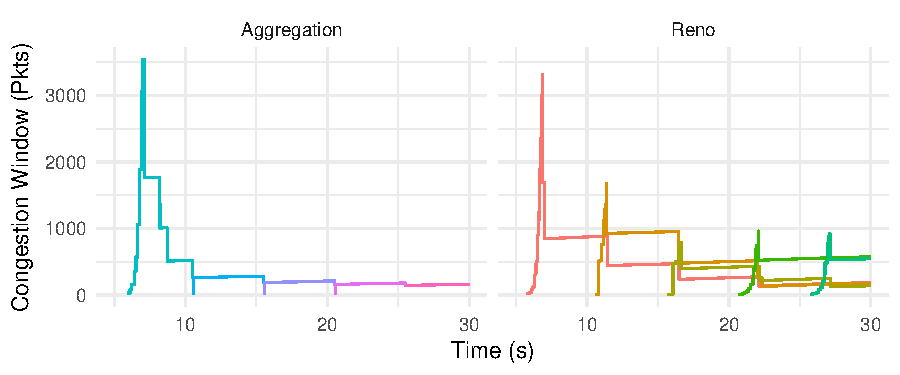
\includegraphics[width=\columnwidth]{img/stair}
    \caption{$5$ 20-second iperf flows with $10$ second staggered starts. While Reno (right) must individually probe for bandwidth for each new connection, an aggregating congestion controller is able to immediately set the connection's congestion window to the fair share value.}
    \label{fig:cap:agg}
\end{figure}
\begin{figure*}[t!]
    \centering
    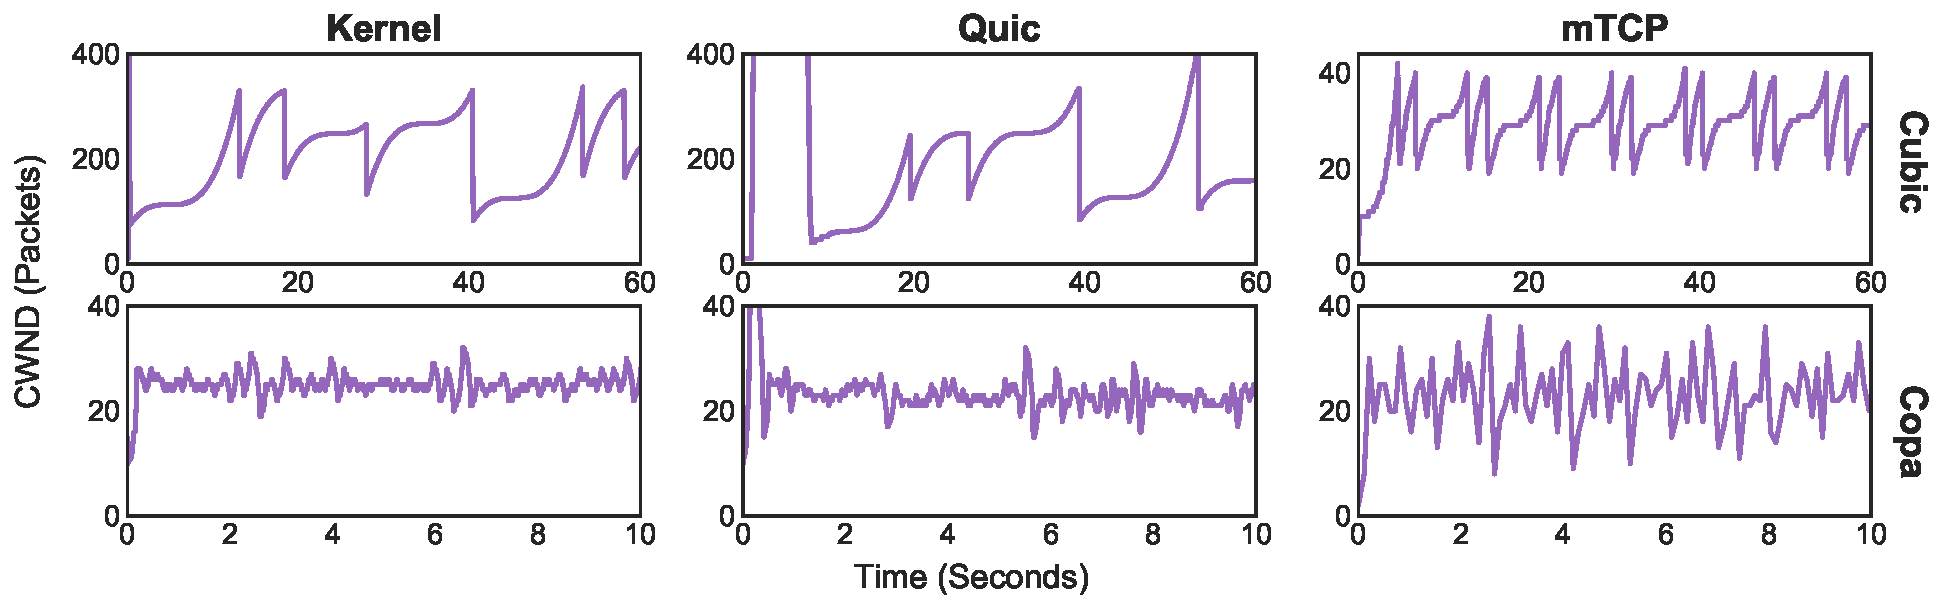
\includegraphics[width=2\columnwidth]{img/datapath-compare.pdf}
    \caption{Comparison of \textit{the same} CCP implementation of Cubic and Copa run on three \textit{different} datapaths with a fixed-rate bottleneck link. %The congestion window naturally evolves differently on each datapath, but the characteristic shapes of both algorithms are clearly visible.
    }\label{fig:datapaths:wora}
\end{figure*}

We present four new capabilities enabled by CCP: new classes of congestion control, rapid development and testing of algorithms, congestion control for flow aggregates, and the ability to write an algorithm once and run it on multiple datapaths.

\subsection{New Algorithms}
\label{s:capabilities:algs}

CCP enables a broad new class of congestion control algorithms.
Until now, because congestion control has been embedded in the datapath,
algorithms have been strictly tied to the ACK clock.
As a result, as data rates rise, algorithms have less time to make decisions,
which naturally restricts the computation an algorithm can perform.
By contrast, CCP algorithms are decoupled from the ACK clock.
Although congestion signals must still be acquired and summarized at ever-faster rates, CCP algorithms can amortize computation across different time scales, and use sophisticated data structures and computations that may be unwise on datapaths like the kernel.

One such algorithmic technique we propose~\cite{nimbus}, uses CCP to compute Fourier transforms on estimates of cross traffic and infer whether it is elastic (buffer-filling) or not.
A key component of this technique involves sending traffic in an asymmetric sinusoidal pulse pattern and using the sending and receiving rates measured over an RTT to produce a time-series of cross-traffic rates. The method then computes the FFT of this series and infers elasticity if the FFT at particular frequencies is large.

In principle, it may be possible to implement such sinusoidal pulses within the datapath, but computing the FFT is unlikely to be practical both due to the timing requirements of the ACK clock as well as the difficulty of performing complex calculations in restrictive programming environments such as the kernel. Moreover, implementing the transmitter outside the datapath in CCP allowed the researchers to iterate through many ideas more quickly than if they had to write kernel code.
%Figure~\ref{fig:capabilities:nimbus-example} shows this pulse pattern and the result of the FFT computation.
We anticipate that in the future, CCP will enable the use of other similarly powerful but computationally-intensive methods such as neural networks.

\subsection{Velocity of Development}
\label{s:capabilities:velocity}

Copa~\cite{copa} is a recently proposed model-based congestion control algorithm that seeks to maintain a target rate that is inversely proportional to the queuing delay, estimated as the difference of the current RTT and the minimum RTT.
Under three network models, this is shown to provide quantifiably low delay, and fair and efficient allocation of bandwidth.
It is robust to non-congestive loss, buffer-bloat, and unequal propagation delays. It includes mechanisms to provide TCP competitiveness, accurate minimum RTT estimation, and imperfect pacing.

The authors of Copa used CCP to implement Copa recently, and in the process discovered a small bug that produced an erroneous minimum RTT estimate due to ACK compression. They solved this problem with a small modification to the Copa fast path,
and in a few hours were able to improve the performance of their earlier user-space implementation. The improvement is summarized here:\\

    \begin{tabular}{c|c|c}
        Algorithm & Throughput & Mean queue delay \\
        \hline
        Copa (UDP) & 1.3 Mbit/s & 9 ms\\
        Copa (CCP-Kernel) & 8.2 Mbit/s  & 11 ms\\
    \end{tabular}

\smallskip
After the ACK compression bug was fixed in the CCP version, Copa achieves higher throughput on a Mahimahi link with 25 ms RTT and 12 Mbit/s rate while maintaining low mean queueing delay. Because of ACK compression, the UDP version over-estimates the minimum RTT by $5\times$.

\subsection{Flow Aggregation}
\label{s:capabilities:agg}

% from nimbus nsdi submission's intro
Congestion control on the Internet is performed by individual TCP connections. Each connection independently probes for bandwidth, detects congestion on its path, and reacts to it.
This per-connection paradigm for congestion control has served the Internet well for 30 years, but is a poor fit in many modern traffic control scenarios where a large number of nodes exchange traffic between a few sites.
Examples include: traffic between different datacenters~\cite{b4, swan}; traffic between campuses of an organization; traffic between collaborating universities or companies; traffic between a large content provider (e.g., Netflix) and a network with many clients (e.g., a regional ISP); large-scale data backups from an organization to an external site; etc.

A more modest use case is to implement the per-host aggregation proposed by the
Congestion Manager two decades ago~\cite{cm}. We used CCP to develop a
host-level aggregate controller that maintains a single aggregate window or rate
for a group of flows and allocates that to individual flows---{\em all with no
  changes to the non-CCP parts of the datapath.}

%
%Since CCP has visibility into all the flows in the system, it is uniquely positioned as a platform on which users can implement aggregate congestion control.
%In fact, we make a small modification to CCP to support flow aggregation and show that a proof-of-concept implementation can reduce average flow completion times by \an{XXX}\%.

\paragrapha{Interface} In addition to the \texttt{create()} and \texttt{onReport()} event handlers, we introduce two new APIs for aggregate congestion controllers: \texttt{create\_subflow()} and \texttt{aggregateBy()}.
CCP uses \texttt{aggregateBy()} to classify new connections into aggregates. Then, it calls either the existing \texttt{create()} handler in the case of a new aggregate, or the \texttt{create\_subflow()} handler in the case of an already active one.

These handlers are natural extensions of the existing per-flow API; we implemented API support for aggregation in $80$ lines of code in our Rust CCP implementation (\S\ref{sec:eval}).
Algorithms can aggregate flows using the connection 5-tuple, passed as an argument to \texttt{aggregateBy()}.

As a proof of concept, we implement an algorithm which simply aggregates all flows on each of the hosts's interfaces into one aggregate and assigns the window in equal portions to each sub-flow.
Figure~\ref{fig:cap:agg} shows the aggregator instantaneously apportioning equal windows to each flow in its domain.

 
\subsection{Write-Once, Run-Anywhere}
\label{s:capabilities:wora}
\label{s:datapaths:eval}

Correct implementation of congestion control algorithms, especially increasingly complicated recent work, is a significant undertaking.
As a result, new algorithms are often implemented in a single datapath and new datapaths have very few algorithms implemented. 
CCP enables algorithm designers to focus on building and testing a single solid implementation of their algorithm that users can then run on any (supported) datapath. 

%We could immediately run the same implementations of various algorithms, developed with the kernel datapath, on QUIC and mTCP. We demonstrate this write-once, run-anywhere capability by comparing the behavior of TCP Cubic and Copa over all three datapaths.

To exhibit this capability, we ran the same implementation of both Cubic (not currently implemented in mTCP) and Copa (\S\ref{s:capabilities:velocity}, not currently implemented in any major datapath) on the three different datapaths and plot the congestion window evolution over time in Figure~\ref{fig:datapaths:wora}.

\textit{As expected}, the congestion window naturally evolves differently on each datapath, but the characteristic shapes of both algorithms are clearly visible. Copa uses triangular oscillations around an equilibrium of 1 BDP worth of packets (22 in this case), periodically draining the queue in an attempt to estimate the minimum RTT.

%Show \texttt{cwnd} evolution of new algorithms that these datapaths could not previously support. Show how this exhibits the high-level behavior we'd expect from these algorithms (need to ask Venkat about Copa, say something about cubic ramping back up to wmax, then probing max bandwidth).
% We have run Copa and Cubic on all 3 datapaths, the kernel, QUIC and mTCP. We expect the behavior of the same algorithms across datapaths to be different for portions, e.g. slowstart - but the general behavior of each algorithm is 


%\begin{figure}[t]
%\centering
%\begin{subfigure}{.45\columnwidth}
%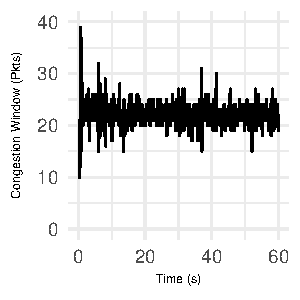
\includegraphics[width=\columnwidth]{img/copa-quic-wora.pdf}
%\subcaption{Copa on Quic}\label{fig:capabilities:wora:copa-quic}
%\end{subfigure}
%
%\begin{subfigure}{.45\columnwidth}
%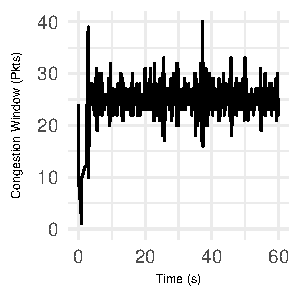
\includegraphics[width=\columnwidth]{img/copa-kernel-wora.pdf}
%\subcaption{Copa on Kernel}\label{fig:capabilities:wora:copa-kernel}
%\end{subfigure}
%
%\begin{subfigure}{.45\columnwidth}
%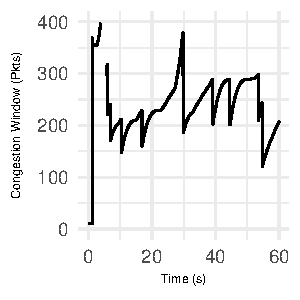
\includegraphics[width=\columnwidth]{img/cubic-quic-wora.pdf}
%\subcaption{Cubic on Quic}\label{fig:capabilities:wora:cubic-quic}
%\end{subfigure}
%
%
%\begin{subfigure}{.45\columnwidth}
%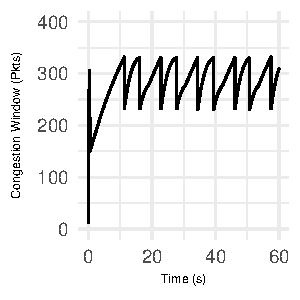
\includegraphics[width=\columnwidth]{img/cubic-kernel-wora.pdf}
%\subcaption{Cubic on Kernel}\label{fig:capabilities:wora:cubic-kernel}
%\end{subfigure}
%
%\caption{Cubic is run on a link with bandwidth 96 Mbps, 20 ms round trip time, and 1 BDP of buffering, for the Kernel and QUIC datapaths. %As Copa performs better at lower link rates, Copa is run on a link with bandwidth 12 Mbps, 20 ms round trip time, and 1 BDP buffering, for %all three datapaths. }\label{fig:capabilities:wora}
%\end{figure}

\section{Evaluation}
\label{sec:eval}
\begin{figure}[t]
\centering
    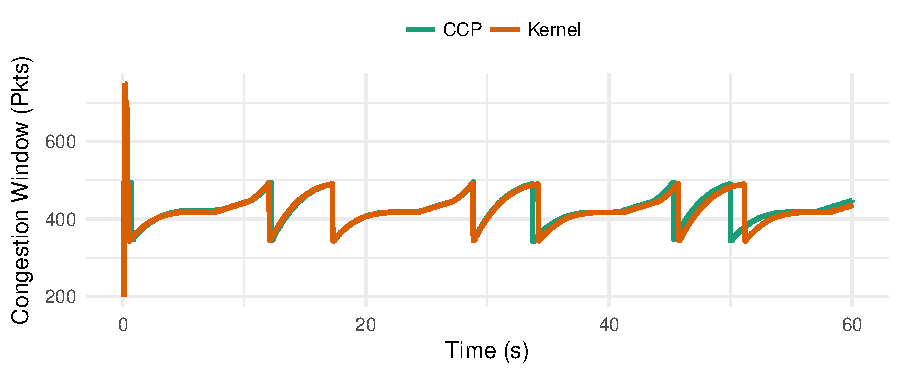
\includegraphics[width=\columnwidth]{img/cubic-3-cwnd-evo-new}
    \caption{Cubic in CCP matches Cubic in Linux TCP.}\label{fig:eval:fidelity:time}
\end{figure}

\noindent
We evaluated the following aspects of CCP:

\paragrapha{Fidelity (\S\ref{sec:eval:fidelity})} Do algorithms implemented in CCP behave similarly to algorithms implemented within the datapath? Using the Linux kernel datapath as a case study, we explore both achieved throughput and delay for persistently backlogged connections as well as achieved flow completion time for dynamic workloads.

\paragrapha{Overhead of datapath communication (\S\ref{sec:eval:whyfold})} How expensive is communication between CCP and the datapath?

\paragrapha{High bandwidth, low RTT (\S\ref{sec:eval:lowrtt})} We use ns-2 simulations to demonstrate that CCP's method of taking congestion control actions periodically can perform well even in ultra-low RTT environments.

%beyond the scenario in \S\ref{sec:eval:whyfold:scale}.
\smallskip
Unless otherwise specified, we evaluated our implementation of CCP using Linux $4.14.0$ on a machine with four $2.8$ Ghz cores and $64$ GB memory. 

\subsection{Fidelity}
\label{sec:eval:fidelity}

The Linux kernel is the most mature datapath we consider. Therefore, we present an in-depth exploration of congestion control outcomes comparing CCP and native-kernel implementations of two widely used congestion control algorithms: NewReno~\cite{newreno} and Cubic~\cite{cubic}.
As an illustrative example, Figure~\ref{fig:eval:fidelity:time} shows one such comparison of congestion window update decisions over time on an emulated $96$ Mbit/s fixed-rate Mahimahi~\cite{mahimahi} link with a $20$ ms RTT.
We expect and indeed observe minor deviations as the connection progresses and small timing differences between the two implementations cause the window to differ, but overall,
not only does CCP's implementation of Cubic exhibit a window update consistent with a cubic increase function, but its updates closely match the kernel implementation.

For the remainder of this subsection, we compare the performance of CCP and kernel implementations of NewReno and Cubic on three metrics (throughput and delay in \S\ref{sec:eval:fidelity:tput-delay}, and FCT in \S\ref{sec:eval:fidelity:fct}) and three scenarios, all using Mahimahi.

\subsubsection{Throughput and Delay.}
\label{sec:eval:fidelity:tput-delay}

We study the following scenarios:

\paragrapha{Fixed-rate link (``fixed'')} A 20 ms RTT link with a fixed $96$ Mbit/s rate and 1 BDP of buffering.

\paragrapha{Cellular link (``cell'')} A 20 ms RTT variable-rate link with a 100-packet buffer based on a Verizon LTE bandwidth trace~\cite{mahimahi}.

\paragrapha{Stochastic drops (``drop'')} A 20 ms RTT link with a fixed $96$ Mbit/s rate, but with $0.01$\% stochastic loss and an unlimited buffer. To ensure that both tested algorithms encountered exactly the same conditions, we modified Mahimahi to use a fixed random seed when deciding whether to drop a packet.

These three scenarios represent a variety of environments congestion control algorithms encounter in practice, from predictable to mobile to bufferbloated paths. We calculate, per-RTT over twenty 1-minute experiments, the achieved throughput (\ref{fig:eval:fidelity:tput-cdf}) and delay (\ref{fig:eval:fidelity:delay-cdf}), and show the ensuing distributions in Figure~\ref{fig:eval:fidelity:cdfs}.

Overall, both distributions are close, suggesting that CCP's implementations make the same congestion control decisions as the kernel.

\begin{figure}[t]
\centering
\begin{subfigure}{\columnwidth}
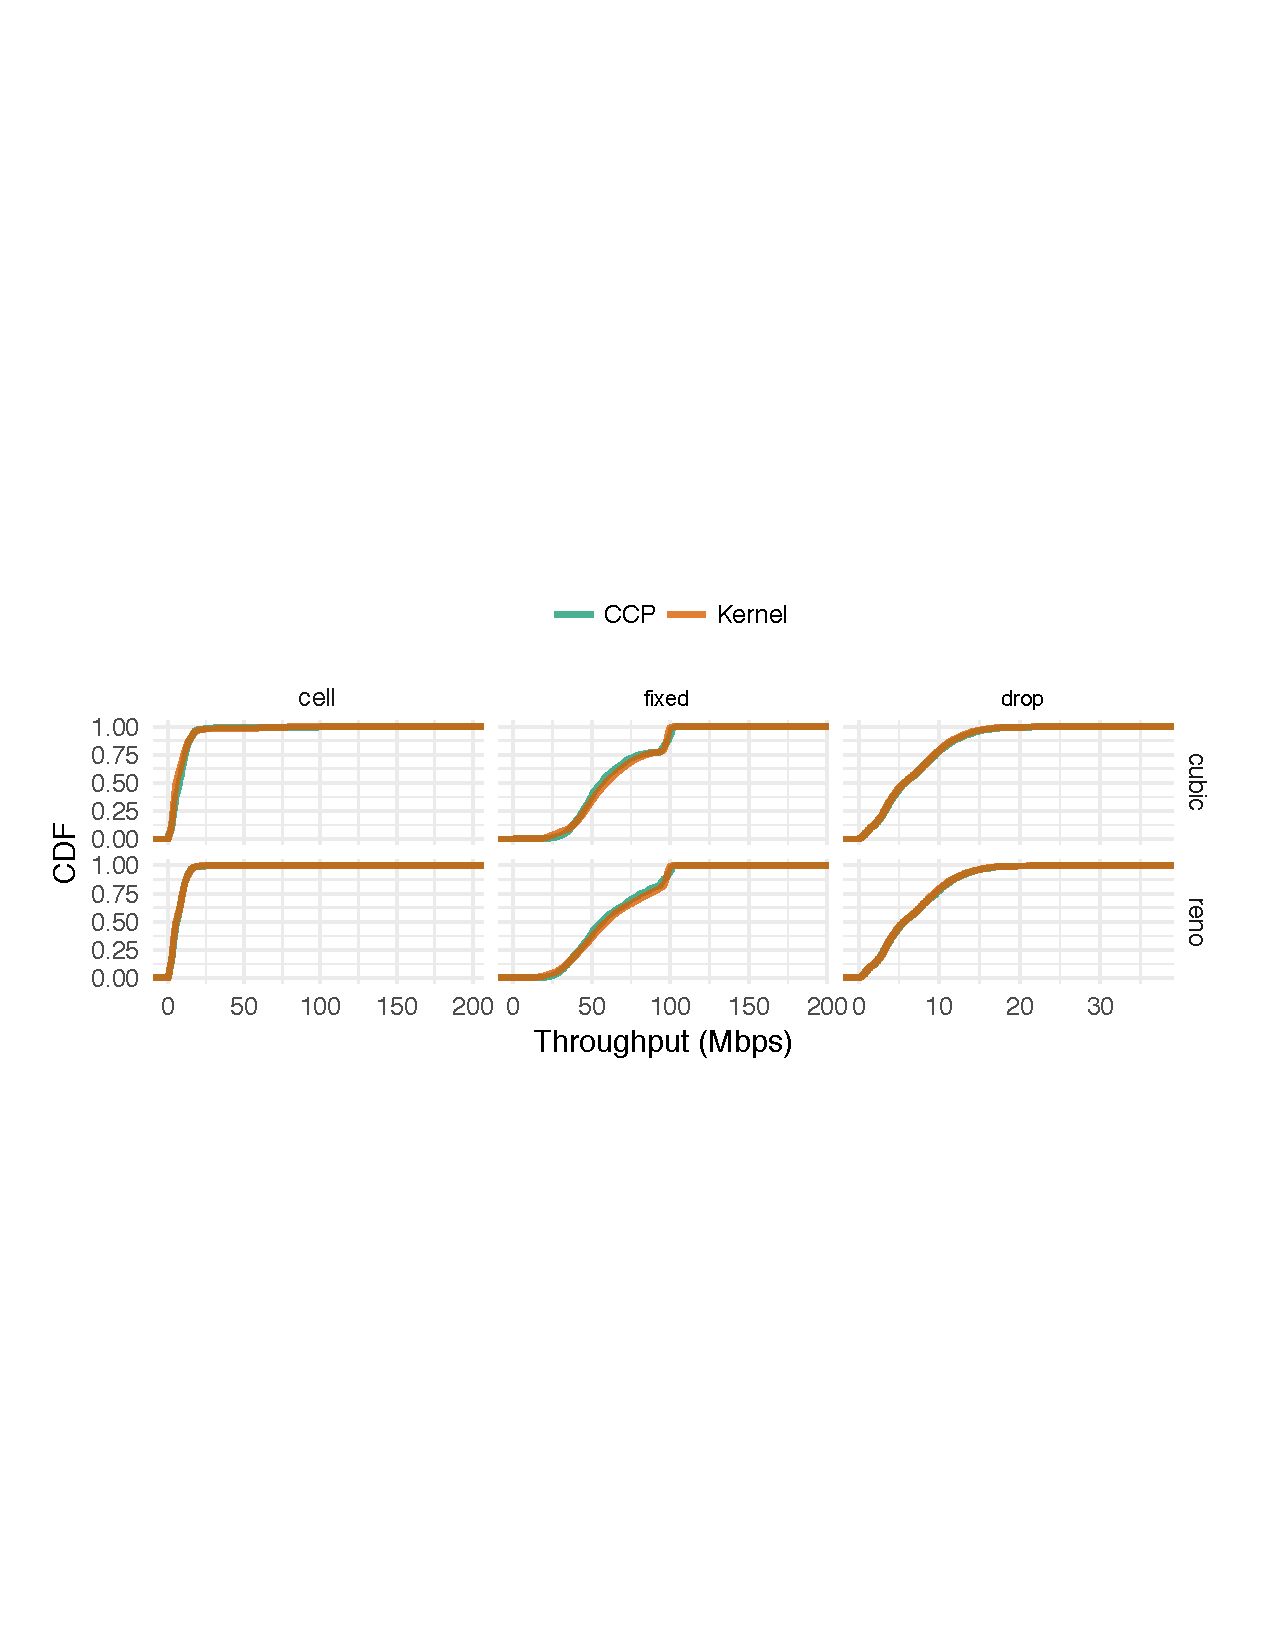
\includegraphics[width=\columnwidth]{img/throughput-cdf-flat}
\subcaption{Achieved throughput over 1 RTT periods. Note the different scales on the x-axes for the three scenarios.}\label{fig:eval:fidelity:tput-cdf}
\end{subfigure}
%
\begin{subfigure}{\columnwidth}
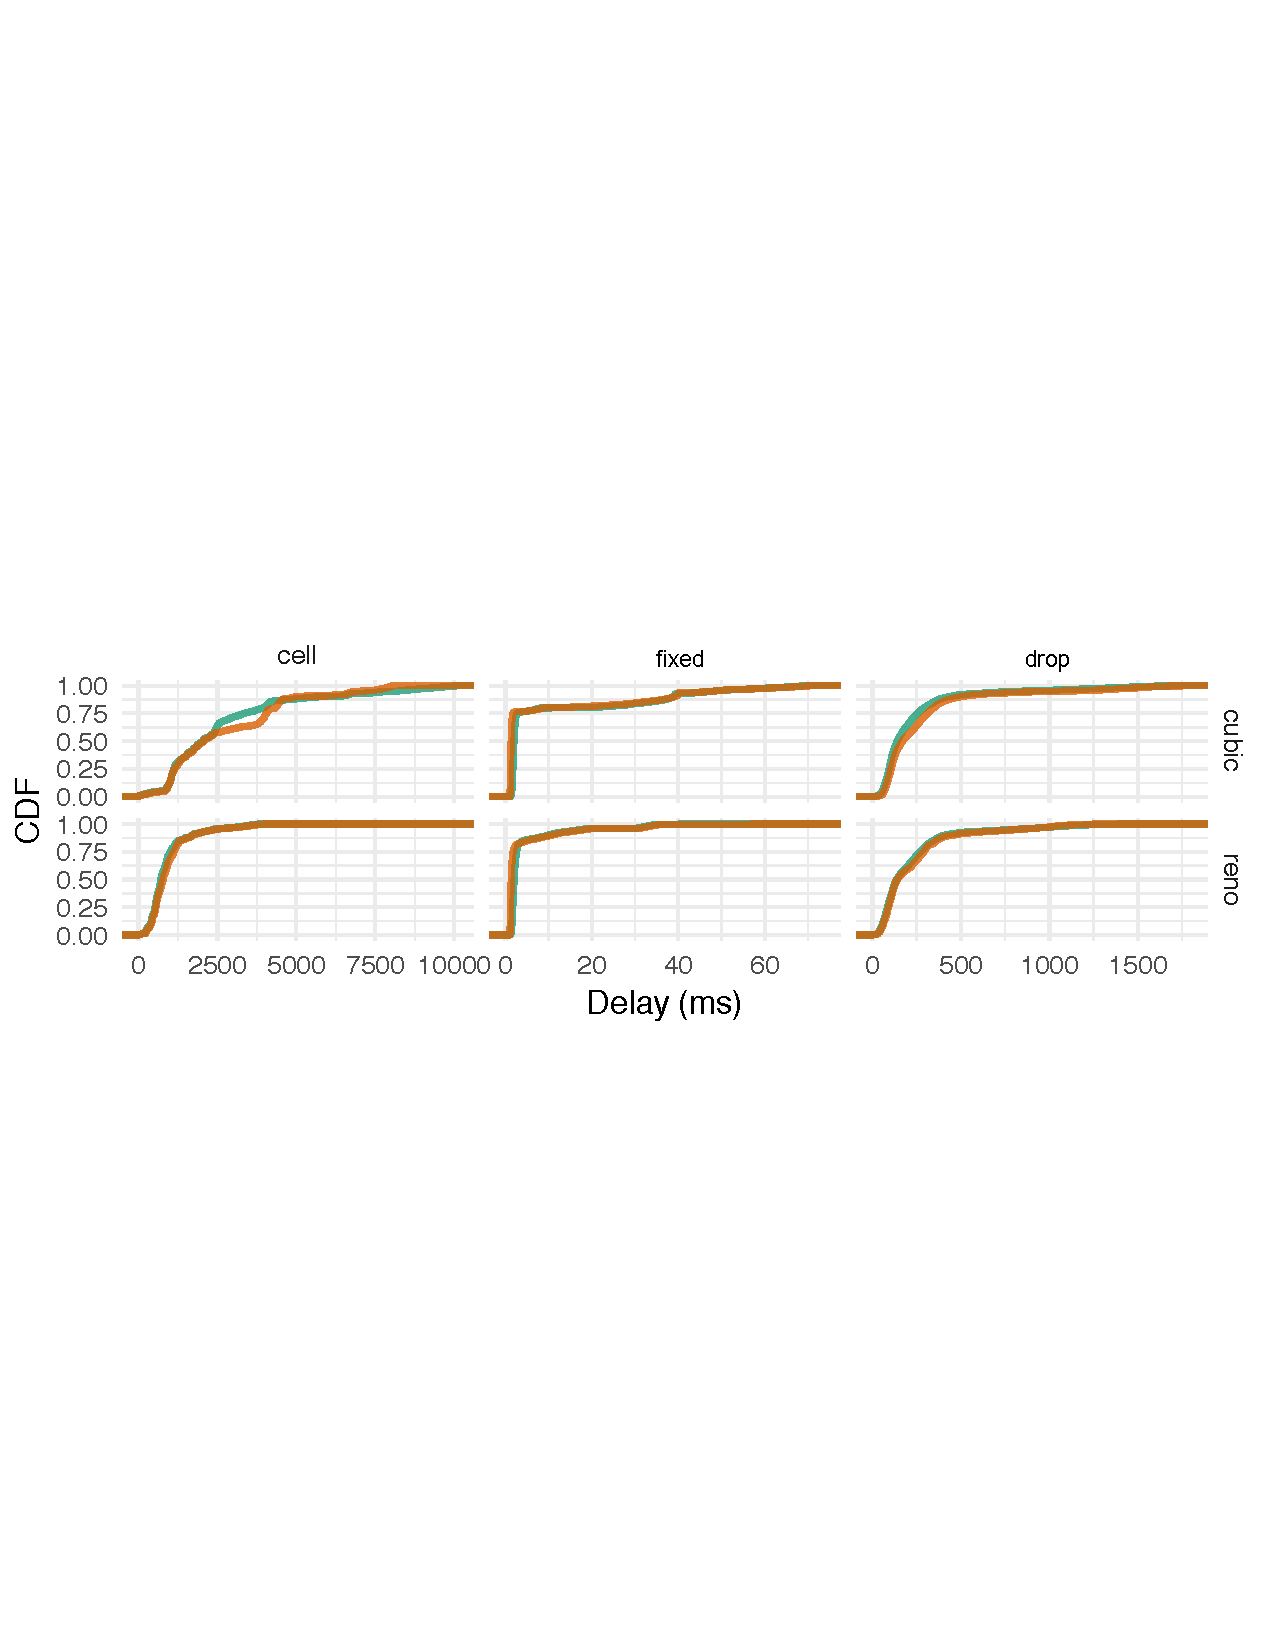
\includegraphics[width=\columnwidth]{img/delay-cdf-flat}
\subcaption{Achieved queueing delay over 1 RTT periods. Note the varying scales on the x-axes for the three scenarios.}\label{fig:eval:fidelity:delay-cdf}
\end{subfigure}
%
\caption{Comparison of achieved throughput over 20 ms periods. The achieved throughput distributions are nearly identical across the three scenarios and two congestion control algorithms evaluated.}\label{fig:eval:fidelity:cdfs}
\end{figure}

\subsubsection{Flow Completion Time.}
\label{sec:eval:fidelity:fct}

\begin{figure}[t]
\centering
\begin{subfigure}{\columnwidth}
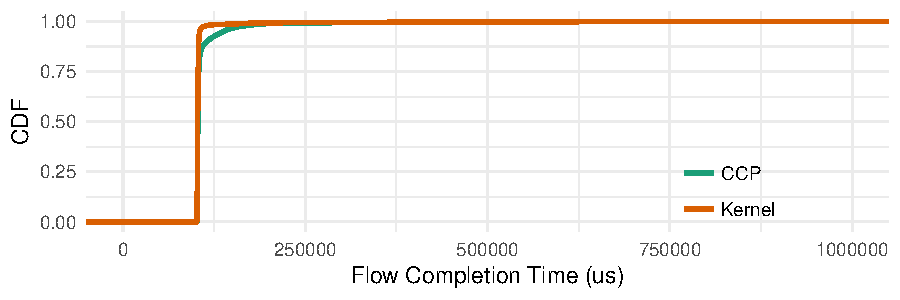
\includegraphics[width=\columnwidth]{img/small_fcts}
\subcaption{0-10KB Flows}\label{fig:eval:fidelity:fct:sml}
\end{subfigure}
%
\begin{subfigure}{\columnwidth}
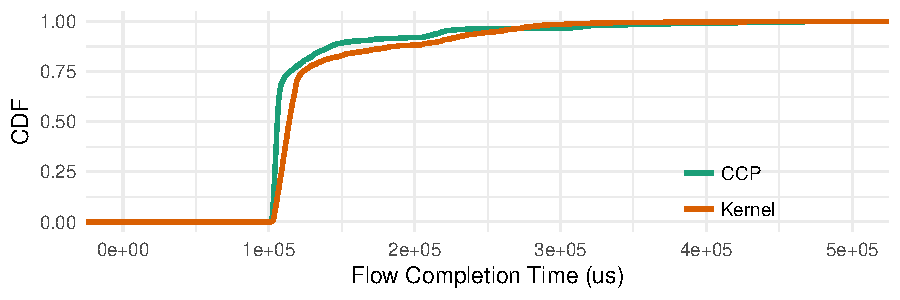
\includegraphics[width=\columnwidth]{img/med_fcts}
\subcaption{10KB-1MB Flows}\label{fig:eval:fidelity:fct:med}
\end{subfigure}
%
\begin{subfigure}{\columnwidth}
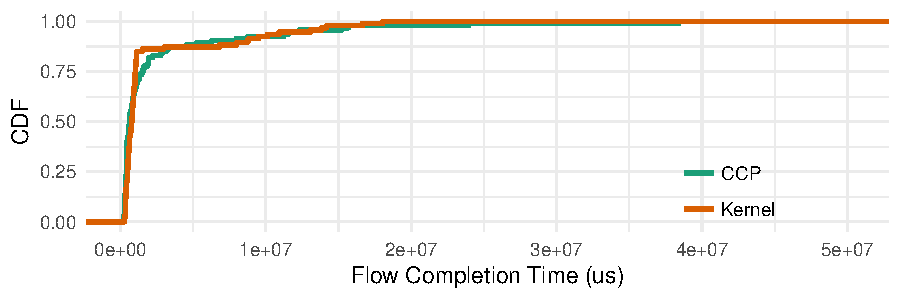
\includegraphics[width=\columnwidth]{img/big_fcts}
\subcaption{1MB+ Flows}\label{fig:eval:fidelity:fct:big}
\end{subfigure}
%
\caption{CDF comparisons of flow completion times. Note the differing x-axes.}\label{fig:eval:fidelity:fct}
\end{figure}

To measure flow completion times (FCT), we use a flow size distribution compiled from CAIDA Internet traces~\cite{caida} in a similar setting to the ``fixed'' scenario above; we use a $100$ ms RTT and a $192$ Mbit/s link.
To generate traffic, we use a traffic generator to sample flow sizes from the distribution and send flows of that size according to a Poisson  arrival process to a single client behind the emulated Mahimahi link. We generate flows with 50\% average link load, and generate $100,000$ flows to the client from $50$ sending servers using persistent connections to the client.
We used Reno as the congestion control algorithm in both cases. To ensure that the kernel-native congestion control ran under the same conditions as the CCP implementation, we disabled the slow-start-after-idle option.

Of the $100,000$ flows we sampled from the CAIDA workload, $97,606$ were $10$ KB or less, comprising $487$ MB, while the $95$ flows greater than $1$ MB in size accounted for $907$ MB out of the workload's total of $1.7$ GB.

Across all flow sizes, CCP achieves FCTs 0.02\% lower than the kernel in the median, 3\% higher in the $75^{\text{th}}$ percentile, and $30$\% higher in the $95^{\text{th}}$ percentile.

\paragrapha{Small flows} Flows less than $10$ KB in size, shown in Figure~\ref{fig:eval:fidelity:fct:sml}, are essentially unaffected by congestion control. These flows, the vast majority of flows in the system, complete before either CCP algorithms or kernel-native algorithms make any significant decisions about them.

\paragrapha{Medium flows} Flows between $10$ KB and $1$ MB in size, in Figure~\ref{fig:eval:fidelity:fct:med}  achieve $7\%$ lower FCT in the median with CCP because CCP slightly penalizes long flows due to its slightly longer update period, freeing up bandwidth for medium size flows to complete.

\paragrapha{Large flows} CCP penalizes some flows larger than $1$ MB in size compared to the native-kernel implementation: $22$\% worse in the median (Figure~\ref{fig:eval:fidelity:fct:big}).

\subsection{Performance}
\label{sec:eval:whyfold}

\subsubsection{Measurement Staleness.}
\label{sec:eval:whyfold:stale}
\begin{figure}[t]
\centering
    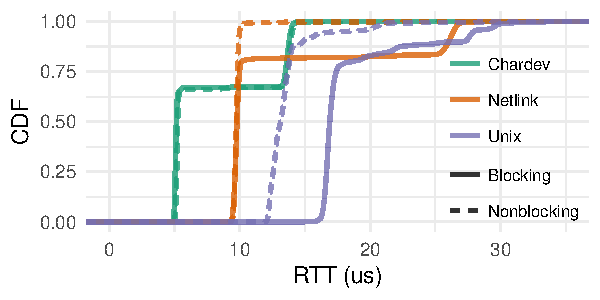
\includegraphics[width=\columnwidth]{img/ipc}
    \caption{Minimum time required to send information to the datapath and receive a response using different IPC mechanisms.}\label{fig:eval:ipc-latency}
\end{figure}

Because our CCP implementation, Portus, runs in a different address space than datapath code, there is some delay between the datapath gathering a report and algorithm code acting upon the report.
In the worst case, a severely delayed measurement could cause an algorithm to make an erroneous window update.

Fortunately, as Figure~\ref{fig:eval:ipc-latency} shows, this overhead is small. We calculate an IPC RTT by sending a time-stamped message to a kernel module (or \userspace{} process in the case of a Unix-domain socket). The receiver then immediately echoes the message, and we measure the elapsed time at the originating process.

We test three IPC mechanisms: Unix-domain sockets~\cite{unix-domain}, a convenient and popular IPC mechanism used for communication between \userspace{} processes; Netlink sockets~\cite{netlink}, a Linux-specific IPC socket used for communication between the kernel and \userspace{}; and a custom kernel module, which implements a message queue that can be accessed (in both \userspace{} and \kernelspace{}) via a character device.
% a custom character device, which can be read from and written to in both \userspace{} and \kernelspace{}.
%our custom kernel module, which implements a message queue that processes (or the kernel) can use via a character device.
% that processes can read from and write to.

In all cases, the $95^{\text{th}}$ percentile latency is less than $30$ $\mu$s. 

\begin{figure*}[t]
\centering
    \begin{subfigure}{0.48\textwidth}
        \centering
        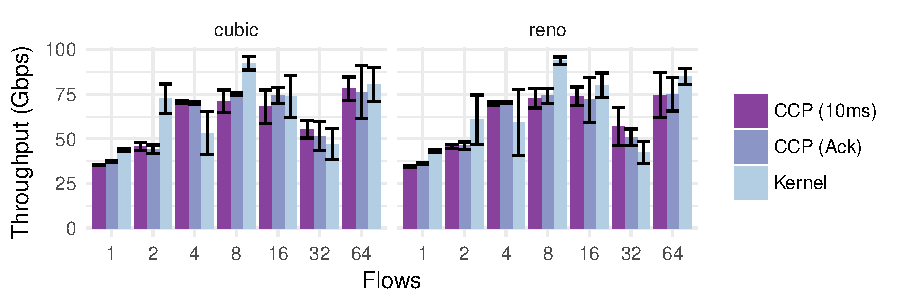
\includegraphics[width=\columnwidth]{img/tputs}
        \subcaption{Achieved localhost throughput as the number of flows increases}\label{fig:eval:perf:numflows}
    \end{subfigure}
    \begin{subfigure}{0.48\textwidth}
        \centering
        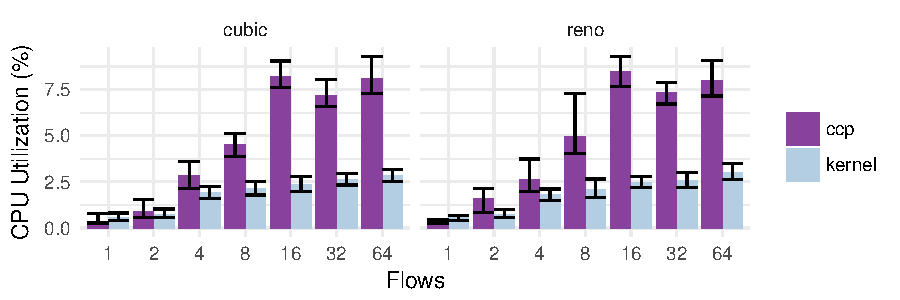
\includegraphics[width=\columnwidth]{img/10G_cpu_util_new}
        \subcaption{CPU Utilization when saturating a 10 Gbit/s link.}\label{fig:eval:perf:10g}
    \end{subfigure}
    \caption{CCP can handle many concurrent flows without significant CPU overhead. Error bars show standard deviation.}\label{fig:eval:perf}
\end{figure*}

\begin{figure}
    \centering
    \begin{subfigure}{\columnwidth}
    \centering
    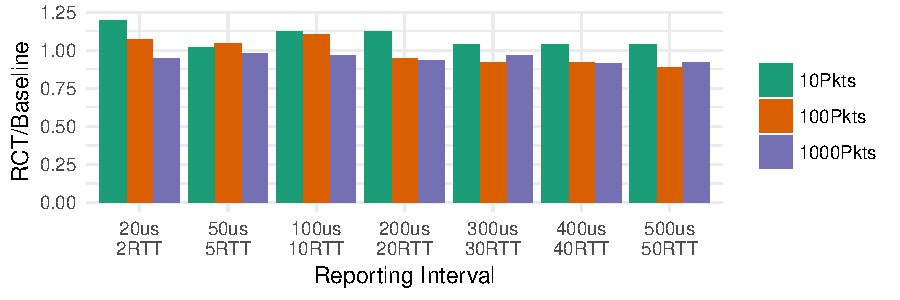
\includegraphics[width=\columnwidth]{img/10g-rct}
    \subcaption{Tail flow completion time at 10 Gbit/s}\label{fig:eval:lowrtt:10g}
    \end{subfigure}
    \begin{subfigure}{\columnwidth}
    \centering
    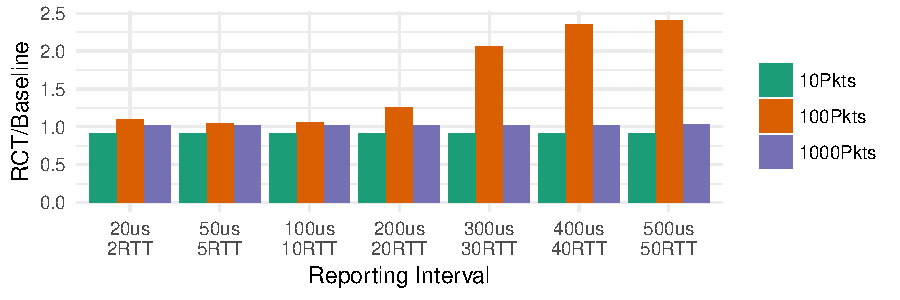
\includegraphics[width=\columnwidth]{img/40g-rct}
    \subcaption{Tail flow completion time at 40 Gbit/s}\label{fig:eval:lowrtt:40g}
    \end{subfigure}
    \caption{Mean tail completion across 50 simulations. While at 10 Gbit/s even rare reporting (every 50 RTTs) has limited overhead (at most 20\%), at 40 Gbit/s, a 1 ms reporting period is necessary to avoid performance degradation.}
    \label{fig:eval:lowrtt}
\end{figure}

\subsubsection{Scalability.}
\label{sec:eval:whyfold:scale}

CCP naturally has nonzero overhead since more context switches must occur to make congestion control decisions in user-space.
We test two scenarios as the number of flows in the system increases exponentially from $1$ to $64$.
In both scenarios, we test CCP's implementation of Reno and Cubic against the Linux kernel's. We measure average throughput and CPU utilization in $1$ second intervals over the course of $10$ $30$-second experiments using iperf~\cite{iperf}. We evaluate CCP with two fold functions: one which implements a reporting interval of $10$ ms, and another which reports on every packet.

We omit mTCP and QUIC from these scalability micro-benchmarks and focus on the kernel datapath. The QUIC toy server is mainly used for integration testing and does not perform well as the number of flows increase; we confirmed this behavior with Google's QUIC team. Similarly, after discussion with the mTCP authors, we were unable to run mTCP at sufficient speeds to saturate a localhost or 10 Gbit/sec connection.

\paragrapha{Localhost microbenchmark} We measure achieved throughput on a loopback interface as the number of flows increases. As the CPU becomes fully utilized, the achieved throughput will plateau. Indeed, in Figure~\ref{fig:eval:perf:numflows}, CCP matches the kernel's throughput up to the maximum number of flows tested, 64. 
%\ma{we said that we tested up to 1024 flows at the beginning of this section. but the results are up to 64 flows?}

\paragrapha{CPU Utilization} To demonstrate the overhead of CCP in a realistic scenario, we scale the number of flows over a single $10$ Gbit/s link between two physical servers and measure the resulting CPU utilization.
Figure~\ref{fig:eval:perf:10g} shows that as the number of flows increases, the CPU utilization in the CCP case rises steadily. The difference between CCP and the kernel is most pronounced in the region between $16$ and $64$ flows, where CCP uses $2.0\times$ as much CPU than the kernel on average; the CPU utilization nevertheless remains under 8\% in all cases.

In both the CPU utilization and the throughput micro-benchmarks, the differences in CPU utilization stem from the necessarily greater number of context switches as more flows send measurements to CCP. Furthermore, the congestion control algorithm used does not affect performance.

\subsection{Low-RTT and High Bandwidth Paths}
\label{sec:eval:lowrtt}

To demonstrate it is feasible to separate congestion control from the datapath even in low-RTT and high bandwidth situations, we simulate a datacenter incast scenario using ns-2~\cite{ns2}.
We model CCP by imposing both forms of delays due to CCP: (i) the period with which actions can be taken (the reporting period) and, (ii) the staleness after which sent messages arrive in CCP. We used our microbenchmarks in \S\ref{sec:eval:whyfold:stale} to set the staleness to 20~$\mu$s, and vary the reporting interval since it is controlled by algorithm implementations. 
We used a $20$ $\mu$s RTT with a 50-to-1 incast traffic pattern across $50$ flows with link speeds of $10$ and $40$ Gbit/s. To increase the statistical significance of our results, we introduce a small random jitter to flow start times ($<$10$ \mu$s with 10 Gbit/s bandwidth and $<$2.5 $\mu$s with 40 Gbit/s bandwidth) and run each point $50$ times with a different simulator random seed value and report the mean.

Figure~\ref{fig:eval:lowrtt} compares the results with the baseline set to in-datapath window update. 
%At $10$ Gbit/s, the tail completion time is within $10$\% of that of an in-datapath update across all request sizes; at $40$ Gbit/s, the tail completion time is within $40$\% of the baseline. 
We find that at $10$ Gbit/s, CCP performance stays within $15$\% of the baseline across different flow sizes and reporting intervals ranging from $10$ $\mu$s to $500$ $\mu$s. 
Recall that $500$ $\mu$s is $50\times$ the RTT; even this infrequent reporting period yields only minor degradation.

Meanwhile, at $40$ Gbit/s the slowdown over the baseline increases with the reporting interval in the case of $100$ packet flows, but not with $10$ or $1000$ packet flows. 
Similar to the results in \S\ref{sec:eval:fidelity:fct}, the short flows and long flows are both unaffected by the reporting period because the short flows complete too quickly and the long flows spend much of their time with large congestion windows regardless of the window update.
Indeed, at $100$ $\mu$s ($10$ RTTs), the tail completion time is within $10$\% of the baseline; as the reporting increases, the tail completion time increases to over $2\times$ the baseline. 
This nevertheless suggests that when reporting intervals are kept to small multiples of the RTT, tail completion time does not suffer.

\section{Conclusion}
\label{s:concl}

We described the design, implementation, and evaluation of CCP, a system that restructures congestion control at the sender. CCP defines better abstractions for congestion control, specifying the responsibilities of the datapath and showing a way to use fold functions and control patterns to exercise control over datapath behavior. We showed how CCP (i) enables the same algorithm code to run on a variety of datapaths, (ii) increases the ``velocity'' of development and improves maintainability, and (iii) facilitates new capabilities such as the congestion manager-style aggregation and sophisticated signal processing algorithms. 

Our implementation achieves high fidelity compared to native datapath implementations at low CPU overhead. The use of fold functions and summarization reduces overhead, but not at the expense of correctness or accuracy.
We additionally showed multiple use cases of CCP, including in Park (\S\ref{s:capabilities:park}) and Bundler (\S\ref{s:capabilities:bundler}).


\label{s:acknowledgements}
\paragrapha{Acknowledgements} We thank
Venkat Arun and the SIGCOMM reviewers for their useful comments and feedback. Special thanks to Eddie Kohler, whose insistence on clarity and brevity greatly improved this paper.
This work was supported in part by DARPA contract HR001117C0048 and NSF grant 1407470.

\bibliographystyle{abbrv}
\bibliography{ccp}
\end{sloppypar}

\end{document}
